\documentclass[journal]{IEEEtran}
\usepackage[utf8]{inputenc}
\usepackage[T1]{fontenc}
\usepackage{graphicx}
\usepackage{amsmath,amssymb}
\usepackage{booktabs}
\usepackage{tabularx}
\usepackage{textcomp}
\usepackage{microtype}
\graphicspath{{figs/}}

\newcommand{\CU}{Coverage-U}
\newcommand{\FB}{Frontier-Bounded}
\newcommand{\RA}{Richness-Angular}

\begin{document}

\title{U-Prioritized Coverage under Finite Mission Budgets: Config-Count
Richness Reduces Residual Bearing-Only Localization Error in UAV Swarms at
Equal Coverage}

\author{Abdelkader~Benmessaoud,~Nabil~Abdelkader~Nouri,~and~Belkacem~Mostefai%
\thanks{The authors are with LASER \& CSAIL, Ziane Achour University of
Djelfa, Algeria (e-mail: aek.benmessaoud@univ-djelfa.dz;
n.nouri@univ-djelfa.dz; b.mostefai@univ-djelfa.dz).}}

\markboth{Benmessaoud, Nouri, and Mostefai}{Config-Count Richness Reduces Residual Bearing-Only Localization Error}

\maketitle


\begin{abstract}
We study multi-agent bearing-only localization under limited-range
communication and a \textbf{finite mission budget} --- the setting where
coverage and localization accuracy genuinely compete. Building on the finding
that bounded-horizon geometric movement (\FB, FB) captures most of the coverage
gain attributed to sophisticated uncertainty signals, we ask whether the
\emph{statistical richness} of independent angular observations --- Chao-type
estimators transposed to per-cell angular configuration counts --- can still
\emph{drive} accuracy when the decision axis is \emph{which frontier target to
spend remaining coverage on}, rather than how to move or when to switch modes.

Following a strict preregistered protocol (paired seeds, Wilcoxon +
Holm-Bonferroni, coverage guard, hard validation gate), we report three
documented falsifications and one confirmed effect. Richness as a direct
target-selection signal (Phase-1/E1) and as a mode-switching signal (Deploy-U,
E2/E3) do not beat the FB control, and the E4 primary
\texttt{quality\_auc} --- the binary fraction of cells localized above
threshold --- is null as well: that fraction saturates under finite budgets.
The confirmed effect is on a distinct pre-specified secondary metric,
\texttt{mean\_bound\_final} (the continuous residual CRLB bound at mission end,
tracked since E2/E3): a coherent $n = 10$ signal, reported explicitly as a
discovery rather than a verdict, motivated a separate higher-power
preregistration (E4-CONFIRM, protocol locked before its runs) that promoted it
to primary with pre-specified success criteria. There,
\textbf{continuous U-prioritized coverage} (\CU: an FB target-score weighted by
the local count of angularly under-determined cells, $\lambda=0.5$) reduces the
residual oracle CRLB bound at mission end by a median of \textbf{20.9\%}
relative to FB across four regimes (Holm-significant in three of four, Fisher
combined $p\approx 0$), \textbf{with no coverage regression} and a
corroborating reduction in never-observed cells. Anchored against the Random
floor and the classical occupancy-entropy baselines Entropy-Frac and
Frontier+Entropy ($n=40$ paired),
the config-count family is the only signal family that beats the FB movement
frame on residual bound at equal-or-better coverage: \CU{} reduces it by a
median 20.9\% and \RA{} by 23--32\% across regimes, and \RA{} is the only
method whose advantage survives 20\% obstacle density. The effect is robust
across $\lambda \in [0.25, 2.0]$ (a plateau, not a knife-edge), conditional on
sparse-obstacle environments, and specific to the budget-limited regime: in
unbounded episodes final localization quality is at parity. We interpret the
results as evidence that config-count richness is a reliable state witness
that becomes an operating lever precisely when mission time --- not distance
--- is the scarce resource. A centralized perfect oracle (E5, $n = 40\times2$)
regresses both metrics, and the local-vs-global ladder isolates why: the same
config-count signal reduces the residual bound $\sim$+30\% when scored locally
and regresses when the same under-set is fused globally. Re-running both
oracle signals in \CU's{} own local movement frame (E5-CORRECTED, $n=40$)
confirms the effect is the \emph{signal}, not the oracle's global movement
frame --- evidence that \textbf{locality, not signal strength}, is what makes
the accuracy/coverage trade-off attainable.
\end{abstract}

\begin{IEEEkeywords}
multi-robot exploration, bearing-only localization, CRLB, Chao estimators,
decentralized coverage, finite mission budget.
\end{IEEEkeywords}


\section{Introduction}
Multi-robot exploration has long balanced two objectives: covering an
environment and acquiring information that is useful downstream
\cite{Yamauchi1997, Burgard2005, Lauri2023}. In a growing class of missions ---
localization of RF/audio emitters, passive sensing, structure-from-motion,
cooperative positioning --- the downstream task is itself
\emph{localization}: each cell must be observed from enough independent viewing
directions that a bearing-only estimator becomes well conditioned. In that
setting the geometric spread of observations (angular diversity) is the
quantity that matters, classically measured by GDOP (Geometric Dilution of
Precision) or the Fisher information matrix \cite{Yarlagadda2000, Bishop2004}.

A separate line of work has proposed \emph{information-driven} exploration
signals --- map entropy \cite{Bourgault2002, Stachniss2005}, expected
information gain \cite{Julian2014, Charrow2015}, POMDP-style value
\cite{Bai2014} --- as a replacement or complement to purely geometric frontier
control \cite{Yamauchi1997}. In our internal validation campaign we found that
when these signals are evaluated against a carefully matched
\emph{bounded-horizon geometric control}, most of their apparent gain on pure
coverage is explained by the receding-horizon movement frame itself, not by
the signal. This paper continues that thread: we keep the honest control, and
ask the harder question of whether a localization-relevant uncertainty signal
can add value \emph{within} that control, under a finite mission budget.

The signal we study is unusual: it is borrowed from ecology. The Chao-type
estimators \cite{Chao1984, ChaoLee1992, ChaoYang1993} and related richness
measures estimate the number of unseen species from the counts of singletons
and doubletons. We transpose these estimators to a per-cell \emph{angular
configuration count}: two observations of a cell contribute independent
configurations when their bearing directions differ by more than a tolerance
(greedy clustering), and a cell is under-determined when it has
$\leq 1$ configuration. The transposed singleton/doubleton signal $U$ then
behaves as a local, cheap proxy for ``how much localization work remains
here.''

The contribution of this paper is a \textbf{preregistered, negative-first
evaluation} of whether this signal can be an operating lever, and the
isolation of the one setting where it is:
\begin{itemize}
\item \textbf{C1.} A hard validation gate (Phase 1a): the oracle CRLB bound
correlates with empirical estimator error ($\rho = 0.638$ pooled, gate GO),
and the local richness signal correlates with residual work (E1,
$\rho = 0.73$--$0.82$).
\item \textbf{C2.} Three documented falsifications: richness as
target-selection (E1) and as mode-switching (E2/E3) does not beat the FB
control on the preregistered primaries.
\item \textbf{C3.} A confirmed positive effect: continuous U-prioritized
coverage (\CU, $\lambda = 0.5$) reduces residual oracle CRLB bound at mission
end by a median 20.9\% at equal coverage (E4-CONFIRM, $n=40$), robust to
$\lambda$ (E4-PARETO), specific to budget-limited missions in sparse-obstacle
environments.
\item \textbf{C4.} A clean experimental protocol and tooling: paired seeds,
Holm-corrected Wilcoxon tests, coverage guards, resumable campaigns, and an
evaluation decoupled from the decision signal (global oracle CRLB), anchored
against the classical occupancy-entropy baselines Entropy-Frac and
Frontier+Entropy (Section~VI-F). The full source code and experiment scripts
are publicly available at [repository URL] to ensure reproducibility.
\end{itemize}

The decisive isolation is that \textbf{locality, not signal strength}, is what
makes the accuracy/coverage trade-off attainable: the same config-count
under-set reduces the residual bound by $\sim$+30\% when scored locally and
regresses both metrics when the same under-set is fused globally by a
centralized oracle (E5, Section~VI-I).


\section{Related Work}
This section reviews the main research areas relevant to our work:
frontier-based exploration, information-driven exploration,
localization-aware planning, cooperative localization, and statistical
richness estimation. We position our contribution relative to each.

\subsection{Multi-robot exploration and frontier methods}
Frontier-based exploration \cite{Yamauchi1997, Yamauchi1998} and its
coordinated extensions \cite{Burgard2005, Franchi2009} select targets on the
boundary between explored and unexplored space. Multi-objective and
multi-criteria variants weight frontier targets by distance, utility, or
information \cite{Gonzalez2002, BasilicoAmigoni2011}. Receding-horizon
next-best-view planning \cite{Bircher2016, Bircher2018} formulates target
selection as short-horizon optimization and is the modern state of the art for
geometric exploration; our FB control instantiates exactly this principle and
serves as the movement baseline throughout. More recent decentralized
multi-UAV systems such as RACER \cite{Zhou2023} dispatch large teams under
asynchronous, bandwidth-limited communication, but their objective remains
rapid spatial coverage and workload balance rather than the geometry of the
acquired observations --- the decision axis of the present work.

\subsection{Information-driven exploration}
Information-theoretic exploration maximizes expected information gain or
entropy reduction of the map \cite{Bourgault2002, Stachniss2005, Julian2014,
Charrow2015}; in cooperative settings, decentralized approximations trade
optimality for scalability \cite{Grocholsky2002, Ponda2012}.
Communication-constrained entropy-field exploration shares this idea in fully
distributed settings \cite{Pongsirijinda2025}, ranking targets by frontier and
robot entropy while merging maps only when robots are within range --- close
to our proximity-fusion model. These methods are computationally heavier than
frontier selection \cite{Grocholsky2002, Ponda2012, Lauri2023} and quantify
probabilistic map uncertainty; our work differs in that the operating signal is
neither occupancy entropy nor information gain but the \emph{angular
configuration count} of a bearing-only observation model.

\subsection{Localization-aware planning: GDOP, CRLB, FIM}
Sensor-placement and path-planning for localization are classically cast as
optimizing a scalar function of the Fisher information matrix --- D-optimality
(determinant), A-optimality (trace of the inverse), or GDOP
\cite{Kaplan2017, Ucinski2005, Martinez2006, Krause2008}. For bearing-only
problems the observability conditions \cite{NardoneAidala1981} and
optimal-observer-maneuver results \cite{Passerieux1998, Oshman1999,
Dogancay2012} show that accuracy is governed by baseline geometry, which is
precisely why our CRLB-based evaluation \cite{Cramér1946, Rao1945} and our
angular-diversity signal are principled. At fleet scale, cooperative
dilution-of-precision analysis of UAV swarms \cite{Chen2020} shows the same
geometric principle: the relative configuration of the swarm directly governs
cooperative positioning accuracy, and increasing the number of agents does not
automatically improve localization.

\subsection{Cooperative localization and communication}
Cooperative localization in wireless networks \cite{Patwari2005,
Wymeersch2009} and multi-robot localization \cite{Ristic2004} emphasize the
role of inter-agent measurement fusion. Distributed estimators now operate on
the sensing graph directly: DCL-Sparse \cite{Sagale2024} improves range-only
cooperative localization in noisy, sparse graphs; GNSS-denied UAV swarms rely
on coalition-based relative localization \cite{Ruan2022} and
formation-constrained geometry \cite{Li2026} to bound accuracy; and a
high-precision airborne study reports significant vertical error when the
swarm's relative baselines lack diversity \cite{Liu2026}. Communication
disruptions motivate predictive bidding, where robots estimate the missing
task-allocation information of disconnected teammates \cite{Woosley2021}, and
low-overhead decentralized strategies that exchange only positions and current
target points \cite{Batinovic2020}. We adopt a limited-range proximity-fusion
model (agents exchange maps when within range), which keeps the decision signal
local and makes the centralized oracle (E5) a genuinely informative upper
bound.

\subsection{Statistical richness estimators}
Chao1 and related estimators \cite{Chao1984, ChaoLee1992, ChaoYang1993,
BurnhamOverton1978} estimate species richness from abundance data and are
standard in ecology. Their use as \emph{decision signals for robot
exploration} --- rather than as post-hoc analytics --- is, to the best of our
knowledge, novel; this paper is the first to evaluate them transposed to
angular configurations and under a preregistered falsification protocol.

\subsection{Positioning}
Relative to this literature, the paper makes three moves. First, it evaluates
information signals against a \emph{matched receding-horizon control}, not
against a weak or absent baseline (the dominant failure mode of
information-driven exploration claims). Second, it uses a global oracle CRLB
bound decoupled from the local decision signal, so accuracy claims are not
circular. Third, it is organized around preregistered falsifications: we
report honestly which operating levers failed before claiming the one that
succeeded.


\section{Problem Formulation}
\subsection{System and observation model}
We consider $m$ agents moving on a $100 \times 100$ grid with randomly placed
obstacles (ratio $q \in \{0.05, 0.20\}$); agents do not know the map. At each
time step, agent $i$ at pose $p_i$ obtains, for every traversable cell in a
Chebyshev sensing footprint of radius $F = 5$, a \emph{bearing-only}
observation toward the cell center: a direction $\theta_k$ from the true
geometry. This is the minimal model under which angular diversity is the
currency of localization, and it lets us compute an exact oracle CRLB
(Section~III-C).

\subsection{Independent angular configurations and the richness signal}
For each cell, observations are summarized by a greedy clustering of their
bearing directions: a new direction joins an existing cluster if it lies
within \texttt{ANG\_TOL} = 15$^\circ$ (circular) of the nearest center,
otherwise it starts a new cluster, capped at \texttt{CLUSTER\_CAP} = 8. Each
cluster center is an \emph{independent angular configuration}. A cell with one
configuration is geometrically under-determined (a single bearing gives a
rank-deficient Fisher matrix); a cell with two or more well-separated
configurations is localizable. We transpose the Chao richness vocabulary to
these counts: $F_1/F_2$ are the numbers of cells with exactly one/two
configurations, and the decision signal is
\begin{equation}
U = \min\!\left( \frac{F_1 (F_1 - 1)}{2 (F_2 + 1)},\; \text{cap} \right),
\qquad \alpha = \frac{U}{U + K},
\end{equation}
with the same bias-corrected form and normalization cap used in the coverage
setting \cite{Chao1984}. All decision signals used by policies are computed
from \emph{local} counts (own observations, augmented only by proximity
fusion); the global count and the CRLB oracle are never fed to any policy (no
leakage, enforced by interface and test).

\subsection{Oracle CRLB evaluation metric}
Localization quality is scored by a global oracle: for every traversable cell,
the information matrix from the true observation geometry is
\begin{equation}
J = \sum_k \frac{u_k u_k^{\top}}{\sigma^2 d_k^2},
\end{equation}
with $u_k$ the unit bearing vector to the $k$-th observing pose, $d_k$ the
distance, and $\sigma$ the nominal bearing precision of $1^\circ$. The per-cell
bound is $b = \sqrt{\operatorname{trace}(J^{-1})}$ in grid-cell units. A cell
is \emph{well-localized} when $b \le \texttt{QUALITY\_THRESHOLD} = 1.5$ cells.
The primary continuous accuracy metric is the \emph{mean residual bound} across
traversable cells at mission end, \texttt{mean\_bound\_final} (lower is
better); the binary fraction of well-localized cells is
$\mathrm{quality}(t) = \text{fraction with } b \le \text{threshold}$, sampled
every 25 steps (normalized AUC = \texttt{quality\_auc}).

\subsection{Communication model}
Agents use limited-range communication: two agents within
\texttt{COMM\_RANGE} = $F$ exchange their maps each step (rendezvous-triggered
fusion \cite{Pongsirijinda2025, Batinovic2020}). The decision signal of every
policy is therefore strictly local and temporally stale relative to the true
map --- the honest distributed setting. Evaluation uses the global
accumulator, which is never revealed to policies.

\subsection{Metrics}
We report the preregistered metrics inline:
\begin{itemize}
\item \emph{Coverage}: \texttt{final\_coverage} (\%) of traversable cells
visited, \texttt{coverage\_auc} over the episode.
\item \emph{Localization}: \texttt{quality\_auc}, \texttt{time\_to\_quality},
\texttt{mean\_bound\_final}, \texttt{undetermined\_final} (fraction of
traversable cells never observed).
\item \emph{Dual objective (E2/E3)}: \texttt{steps\_dual} = first step with
coverage $\geq 90\%$ AND quality $\geq 0.9$.
\end{itemize}
All tests are paired by environment seed; gains are median relative
differences; $p$-values are Holm-Bonferroni corrected across regimes.


\section{Methods}
\subsection{Frontier-Bounded control (FB)}
FB selects a target among frontier cells reachable within a bounded BFS
horizon ($H = 8$), preferring the frontier cell that maximizes the
remaining-exploration potential, with deterministic tie-breaking by per-agent
scatter noise; movement is receding-horizon with an exploration fallback.
$H = 8$ was fixed empirically before the preregistered campaign, and the 90\%
coverage threshold is standard in exploration benchmarks
\cite{Yamauchi1997, Burgard2005}. FB uses \emph{no} uncertainty signal: it is
the validated geometric control and the reference against which every
candidate is tested. Its \texttt{steps\_90} matches the geometric baseline
validated in our internal validation campaign.

\subsection{Richness-Angular (E1, target-selection falsification)}
RA scores frontier targets by the transposed richness signal $U$ over the local
config-count map (frontier $\times$ richness weighting) inside the same bounded
frame. It tests whether richness as a \emph{direct target selection} signal
beats FB on localization quality.

\subsection{Deploy-U (E2/E3, mode-switching falsification)}
Deploy-U keeps the FB coverage mode while the known local map is mostly
under-localized (fraction of known cells with $\leq 1$ configuration above
0.30), then switches to a \emph{deploy} mode that orbits the worst known
under-determined cell (approach by bounded BFS, then orbit with viewing-angle
variation to add independent configurations). It tests richness as a
\emph{mode} signal.

\subsection{Coverage-U (E4, continuous prioritization --- proposed method)}
\CU{} does not change mode. Inside the FB frame it replaces the frontier
utility by a continuous target score
\begin{equation}
\mathrm{score}(\text{target}) = \frac{D}{H} - \lambda \cdot
\frac{\texttt{under\_count\_FOV}(\text{target})}{\texttt{FOV\_area}},
\end{equation}
where $D$ is the bounded-BFS distance to the target, $H$ the horizon, and
\texttt{under\_count\_FOV} counts the \emph{known-free cells with $\leq 1$
angular configuration} inside the target's sensing footprint, computed in
$O(1)$ per candidate by an integral image. $\lambda = 0.5$ was fixed before any
campaign (no tuning); $\lambda = 0$ is exactly FB (verified by an
action-identical test). The hypothesis: with a finite mission time, standard
coverage spends the remaining budget on frontier cells that are cheap to reach
but leave residual localization error; biasing target choice toward
under-observed regions buys residual accuracy at the same coverage cost.

\subsection{Dynamic normalization for dense environments (proposed variant)}
One boundary condition found in Section~VI-F motivates a proposed variant of
the score: the \CU{} advantage vanishes at 20\% obstacle density, and part of
the mechanism is signal dilution. The score above normalizes
\texttt{under\_count\_FOV} by the constant square area \texttt{FOV\_area}; in a
fragmented environment a large fraction of that window is blocked, so the same
absolute under-count yields a smaller bonus and the signal is attenuated
precisely where it is needed. The variant replaces the constant denominator by
the number of \emph{traversable} cells (free + unknown) actually inside the
footprint:
\begin{equation}
\mathrm{score}(t) = \frac{D}{H} - \lambda \cdot
\frac{\texttt{under\_count\_FOV}(t)}{\texttt{free\_count\_FOV}(t)},
\end{equation}
which keeps the bonus normalized by what the sensor can actually observe. It
is a two-line change to the integral-image computation and is the first natural
extension to test in dense terrain; it is not run here (it would be a new
preregistered variant) and is returned to in Section~IX.

\subsection{Centralized oracle (E5, control bound)}
E5 defines an infeasible centralized control with perfect map knowledge that
maximizes the same score form using global under-sets --- either the
config-count signal under perfect fusion (CentralOracle-Config) or the true
CRLB bottleneck (CentralOracle-CRLB). It anchors the transposition ratio
$\rho = \mathrm{reduction}(\CU) / \mathrm{reduction}(\text{CentralCRLB})$.
Section~VI-I reports the completed campaign, its diagnostic extension
(coverage-guarded oracle variants, which cannot bind), and the frame-matched
re-run (E5-CORRECTED) that isolates the signal effect.

\subsection{Comparison baselines (occupancy entropy)}
We also compare against classical occupancy-entropy baselines: Entropy-Frac
(fractional entropy gain over the footprint) and Frontier+Entropy (frontier
selection weighted by map entropy) \cite{Bourgault2002, Stachniss2005}. They
run inside the same Frontier-Bounded frame and are introduced here so that the
battery of Section~VI-F reads as a planned comparison rather than a post-hoc
addition.


\section{Experimental Protocol}
\subsection{Preregistration and gates}
Every experiment is preregistered in the repository (\texttt{PRE\_REG\_*.md})
before execution, with locked metrics, thresholds, and verdict rules; the
analysis scripts implement the verdicts exactly and are run unchanged on the
final data. A hard gate (Phase 1a) must pass before any campaign runs: the
oracle CRLB bound must correlate with empirical estimator error, and the local
richness signal must correlate with residual work (Section~VI-A).

\subsection{Regimes and budgets}
Regimes vary the team size and obstacle ratio: A2 (2 UAVs), A3 (3 UAVs), A6
(6 UAVs) at 5\% obstacles, and A6 at 20\% obstacles (A6\_obs020). The finite
budget $T$ per regime is $0.7 \times$ the FB median \texttt{steps\_90}
measured in E3: A2 = 4200, A3 = 3200, A6 = 1600, A6\_obs020 = 1750. At these
budgets coverage is partial (66--76\%), so coverage and accuracy genuinely
compete.

\subsection{Paired design and statistics}
All comparisons are paired at the map level: run index $r$ uses
$\mathrm{env\_seed} = 0 + 1000 \cdot r$ for every method. Significance is
assessed by the paired Wilcoxon signed-rank test; $p$-values are
Holm-Bonferroni corrected across regimes; the matched-pairs delta $m/n^2$ is
reported. Primary/guard/secondary metrics and verdict rules are fixed
per-stage. $n = 10$ pairs for discovery (E1/E2/E3/E4), $n = 40$ for the
confirmation campaign (E4-CONFIRM, E4-PARETO).

\subsection{Experiment map}

\begin{table}[t]
\caption{Experiment map. All stages preregistered; E4-CONFIRM and E4-PARETO fixed $\lambda = 0.5$ and budgets before any data were seen.}
\label{tab:map}
\centering
\begin{tabular}{l c c c c}
\toprule
Stage & Question & Primary & $n$ & Verdict \\
\midrule
Phase 1a & CRLB valid? U predicts residual work? & $\rho$(bound, error) & 10 & GO (gate) \\
E1 & Richness as target selection? & quality\_auc & 10 & FAIL (parity) \\
E2/E3 & Richness as mode switch? & steps\_dual & 10 & FAIL (parity) \\
E4 & U-prioritization under budget? & quality\_auc & 10 & FAIL (parity) $\rightarrow$ discovery on mean\_bound \\
E4-CONFIRM & Confirmation, higher power? & mean\_bound\_final & 40 & PASS \\
E4-PARETO & $\lambda$ robustness? & mean\_bound\_final & 40 & PASS (plateau) \\
E5 & Centralized oracle bound? & mean\_bound\_final & 40 & FAIL (regression) \\
E5-DIAG & Oracle failure: calibration or structure? & mean\_bound\_final & 40 & NEGATIVE STRUCTURE (guard inert) \\
E5-CORRECTED & Local frame + global signal? & mean\_bound\_final & 40 & FAIL (locality confirmed) \\
\bottomrule
\end{tabular}
\end{table}


\section{Results}
\subsection{Phase 1a: metric validation (gate)}
The oracle CRLB bound is a valid accuracy proxy: pooled across 95{,}000 tested
cells (91{,}530 localizable), $\rho(\text{bound, empirical error}) = 
0.638
 on localizable cells ($p < 0.05$, min 0.5), and the local richness
signal correlates negatively with empirical error ($\rho(U\_local, error) = 
-0.457
, max $-0.4$, $p < 0.05$). Both conditions pass and the gate is GO. This
is the evidence that the evaluation metric and the decision signal are both
meaningful indicators of localization work.

\subsection{E1: richness as target selection --- falsified}
In the base scenario (S1: 6 UAVs, FOV 5, unbounded 4500-step episodes), the
three phase-1 methods differ sharply on the movement frame and barely on the
signal. Both FB ($p = 0.002$ vs Random) and RA ($p = 0.002$ vs Random) far
exceed the Random floor, while RA is not significantly better than FB
($p = 0.084$, $-1.5\%$): richness as a target-selection signal is falsified.

\begin{table}[t]
\caption{Phase-1 (E1), 6 UAVs, FOV 5, $n = 10$.}
\label{tab:e1}
\centering
\begin{tabular}{l c c c c}
\toprule
Method & quality\_auc (med [IQR]) & quality\_final & time\_to\_quality & undetermined \\
\midrule
Random & 0.551 [0.493--0.626] & 0.770 & 4150 & 0.2162 \\
Frontier-Bounded & 0.940 [0.939--0.942] & 1.000 & 350 & 0.0000 \\
Richness-Angular & 0.926 [0.918--0.935] & 1.000 & 575 & 0.0000 \\
\bottomrule
\end{tabular}
\end{table}


\begin{figure}[t]
\centering
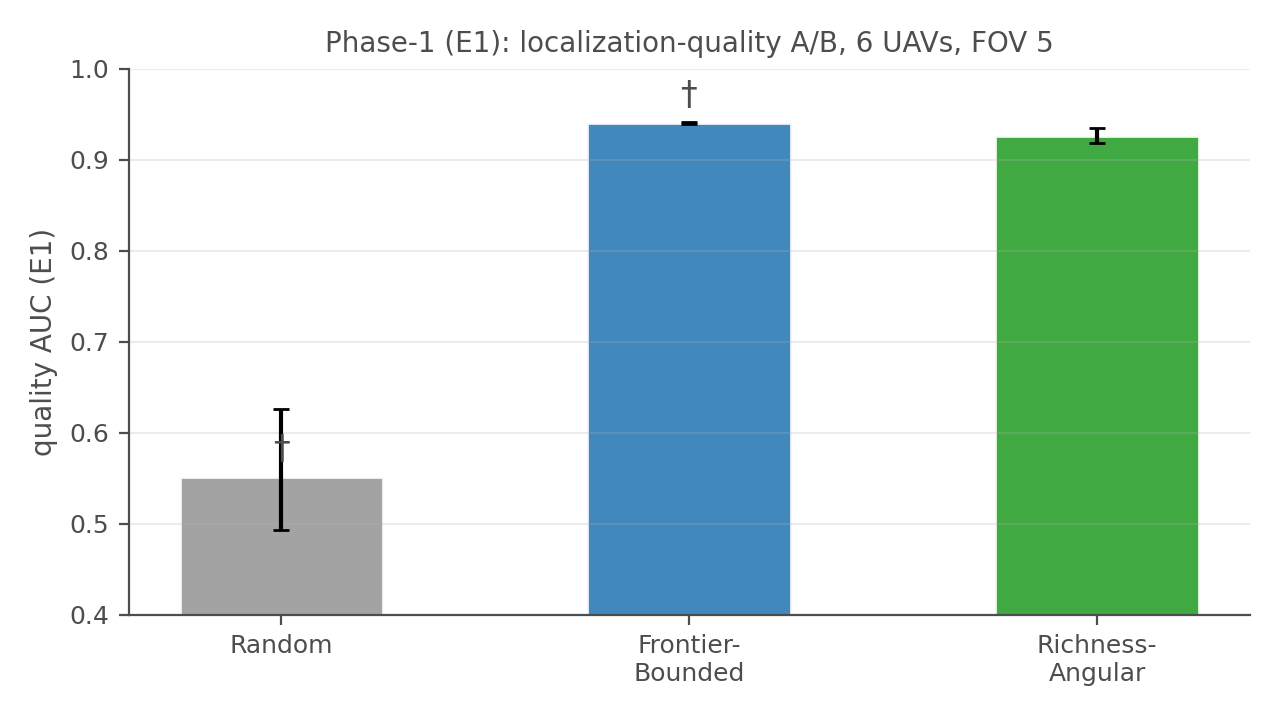
\includegraphics[width=\columnwidth]{fig_paper_phase1.png}
\caption{Phase-1 quality AUC for Random, Frontier-Bounded (FB), and
Richness-Angular (RA) on the unbounded 4500-step scenario ($n = 10$;
$\dagger = p < 0.05$ vs Random).}
\label{fig:phase1}
\end{figure}

\subsection{E2/E3: richness as a mode switch --- falsified}
Deploy-U orbits under-determined cells once the known map is mostly localized.
Its deploy mode fires only 2--6\% of decisions (orbit 0.5--1\%) and never
changes the dual-objective outcome: the median gain on \texttt{steps\_dual} is
$-1.1\%$ (threshold +8\%), with no Holm significance --- richness as a
mode-switching signal is falsified, and final localization quality is at parity
everywhere (quality\_final = 1.0).

\begin{table}[t]
\caption{E2/E3: \texttt{steps\_dual} (first step with coverage $\geq 90\%$ and quality $\geq 0.9$). Gain threshold +8\%.}
\label{tab:e23}
\centering
\begin{tabular}{l c c c c c}
\toprule
Regime & FB steps\_dual & Deploy-U steps\_dual & gain\% & $p$ & $p$\_Holm \\
\midrule
\multicolumn{6}{c}{\textbf{A2 (2 UAVs)}} \\
\midrule
A2 (2 UAVs) & 6000 & 6088 & -1.9 & 0.8203 & 0.8203 \\
\multicolumn{6}{c}{\textbf{A3 (3 UAVs)}} \\
\midrule
A3 (3 UAVs) & 4550 & 4375 & -0.3 & 0.7344 & 0.8203 \\
\multicolumn{6}{c}{\textbf{A6 (6 UAVs)}} \\
\midrule
A6 (6 UAVs) & 2325 & 2450 & -6.4 & 0.2188 & 0.6562 \\
\multicolumn{6}{c}{\textbf{A6, 20\% obs}} \\
\midrule
A6, 20\% obs & 2512 & 2300 & +9.0 & 0.0371 & 0.1484 \\
\bottomrule
\end{tabular}
\end{table}


\begin{figure*}[t]
\centering
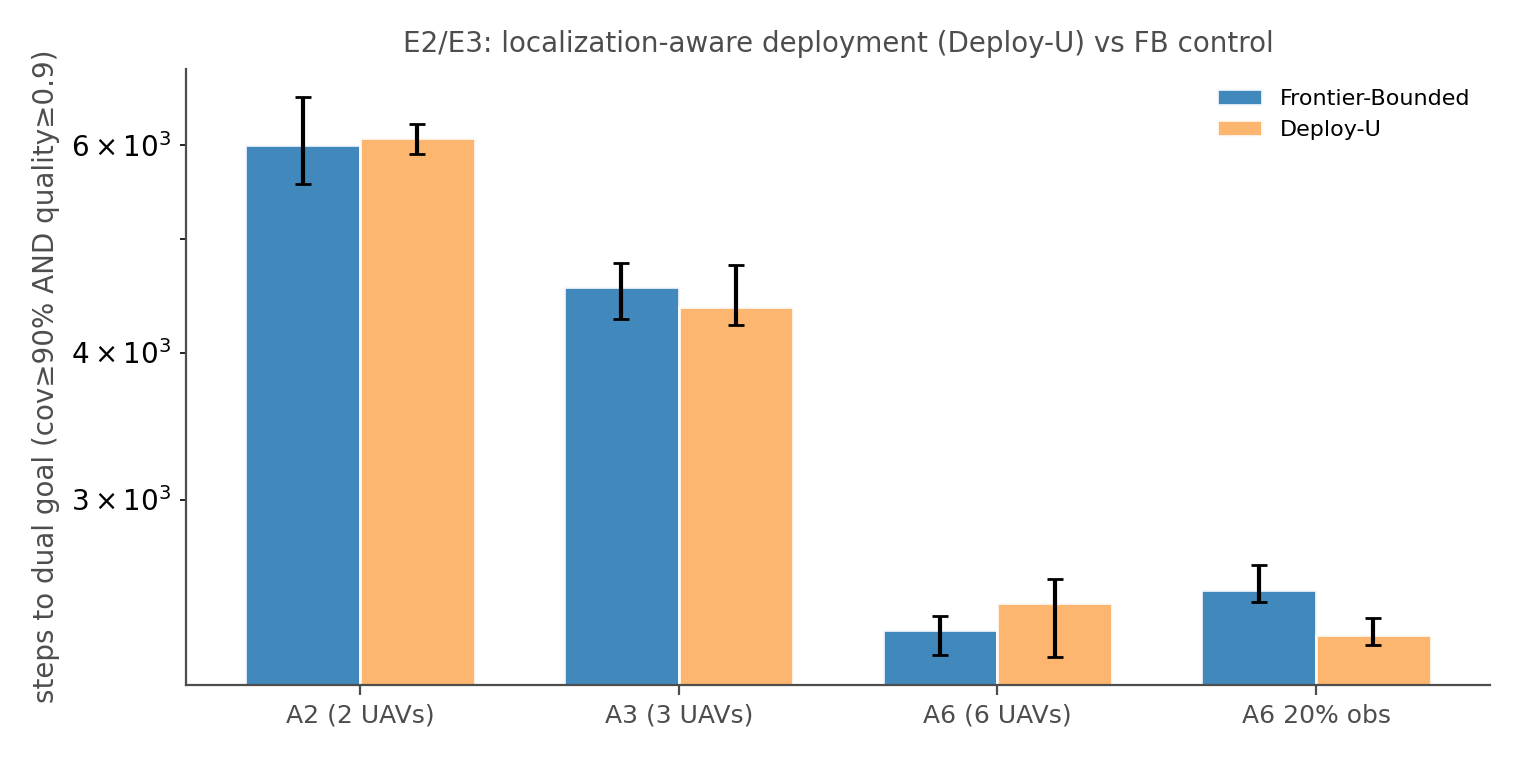
\includegraphics[width=\textwidth]{fig_paper_e3.png}
\caption{E2/E3: dual-objective completion time (log scale).}
\label{fig:e3}
\end{figure*}

\subsection{E4: preregistered primary fails; a consistent secondary discovery}
Under finite budgets, \CU{} ($\lambda = 0.5$) does not move the preregistered
primary \texttt{quality\_auc} (median gain +0.4\%, no Holm significance): the
binary fraction of well-localized cells saturates and cannot see improvements
below the threshold. However, on the continuous accuracy metric
\texttt{mean\_bound\_final} --- a secondary metric pre-specified since E2/E3 ---
the effect is coherent across all four regimes at
$n = 10$ (relative reduction vs FB 13.6--28.3\%, three of four raw $p < 0.05$,
best Holm $p = 0.098$) with no coverage regression. This directional discovery
--- not a verdict --- motivated the higher-power preregistered confirmation
(E4-CONFIRM, protocol locked before its runs).

\subsection{E4-CONFIRM: confirmed reduction at equal coverage (PASS)}
With $n = 40$ paired runs per regime, the residual oracle CRLB bound at mission
end is significantly lower for \CU{} in three of four regimes, with a median
relative reduction of 
20.9
\% and Fisher combined $p \approx 0$. The corroborating reduction in
never-observed cells is also Holm-significant in three of four regimes;
A6\_obs020 is the single non-significant, mildly reversed regime:

\begin{table}[t]
\caption{E4-CONFIRM: \texttt{mean\_bound\_final} at mission end (budget $T$), $n = 40$ paired.}
\label{tab:e4c}
\centering
\begin{tabular}{l c c c c c}
\toprule
Regime & FB bound & CU bound & rel-red\% & $p$ & $p$\_Holm \\
\midrule
\multicolumn{6}{c}{\textbf{A2 (2 UAVs)}} \\
\midrule
A2 (2 UAVs) & 0.0277 & 0.0209 & +24.7 & 0.0002 & 0.0003 \\
\multicolumn{6}{c}{\textbf{A3 (3 UAVs)}} \\
\midrule
A3 (3 UAVs) & 0.0222 & 0.0185 & +17.0 & $<$0.0001 & $<$0.0001 \\
\multicolumn{6}{c}{\textbf{A6 (6 UAVs)}} \\
\midrule
A6 (6 UAVs) & 0.0244 & 0.0181 & +25.7 & $<$0.0001 & $<$0.0001 \\
\multicolumn{6}{c}{\textbf{A6, 20\% obs}} \\
\midrule
A6, 20\% obs & 0.0232 & 0.0219 & +5.4 & 0.2214 & 0.2214 \\
\bottomrule
\end{tabular}
\end{table}


\begin{figure*}[t]
\centering
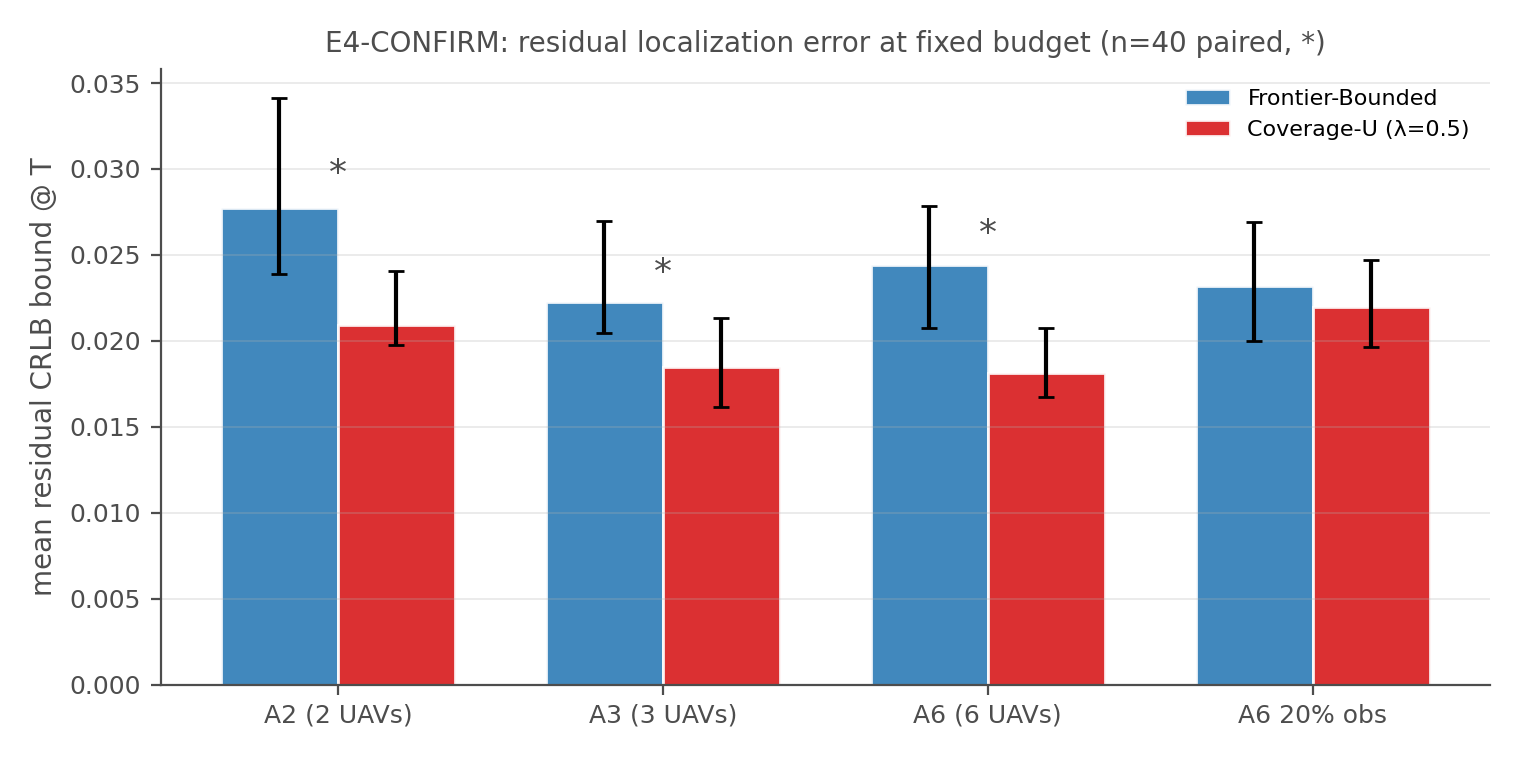
\includegraphics[width=\textwidth]{fig_paper_e4confirm.png}
\caption{E4-CONFIRM: residual CRLB bound at mission end ($* =$
Holm-significant Wilcoxon, $p < 0.05$).}
\label{fig:e4c}
\end{figure*}

\begin{figure*}[t]
\centering
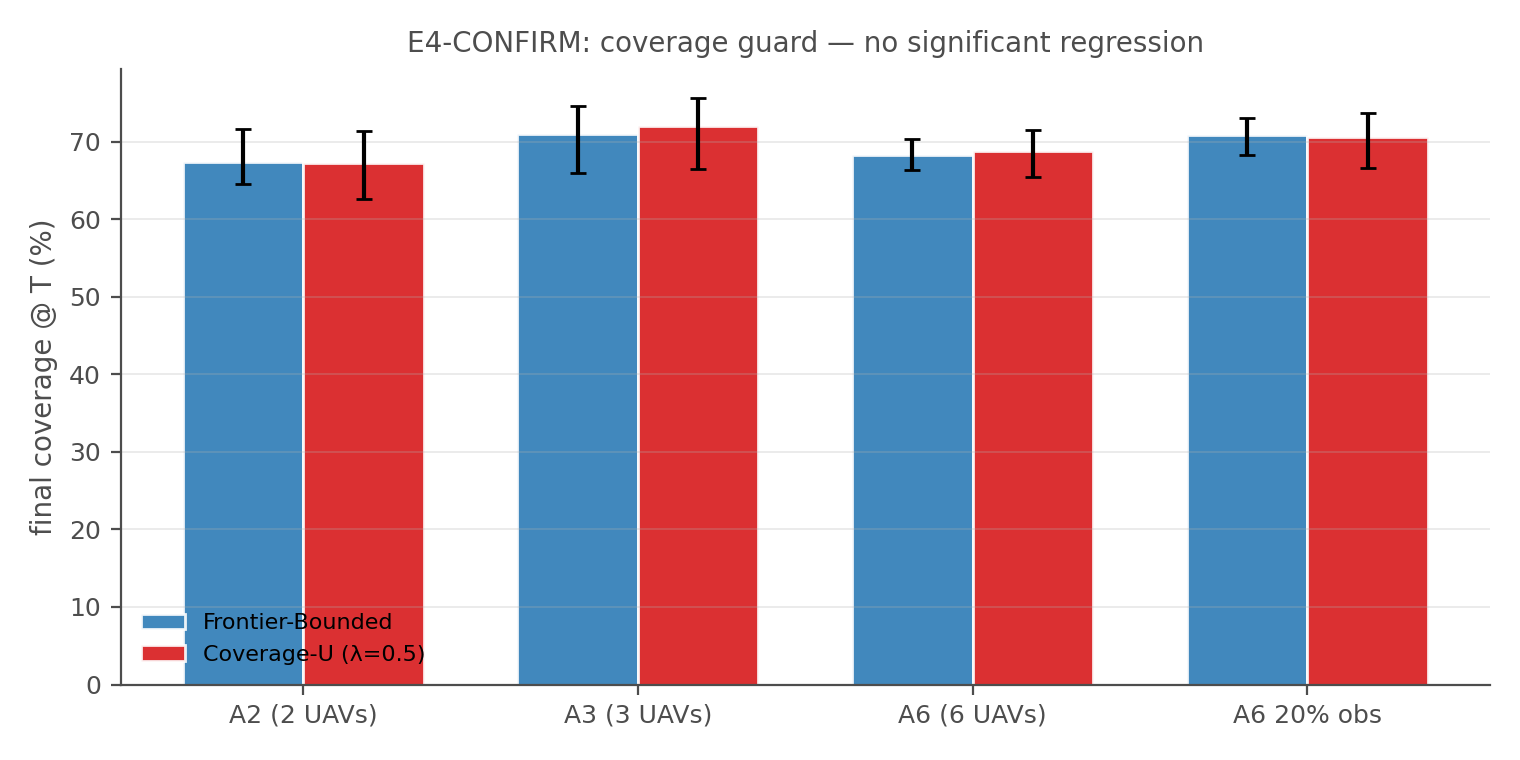
\includegraphics[width=\textwidth]{fig_paper_coverage.png}
\caption{Coverage guard: final coverage at mission end for Frontier-Bounded
(FB) and \CU{} (CU) under finite budgets ($n = 40$).}
\label{fig:guard}
\end{figure*}

\begin{table}[t]
\caption{E4-CONFIRM corroboration: fraction of traversable cells never observed (lower is better).}
\label{tab:undet}
\centering
\begin{tabular}{l c c c c c}
\toprule
Regime & FB undet. & CU undet. & gain\% & $p$ & $p$\_Holm \\
\midrule
\multicolumn{6}{c}{\textbf{A2 (2 UAVs)}} \\
\midrule
A2 (2 UAVs) & 0.0109 & 0.0032 & +71.7 & 0.0170 & 0.0341 \\
\multicolumn{6}{c}{\textbf{A3 (3 UAVs)}} \\
\midrule
A3 (3 UAVs) & 0.0085 & 0.0009 & +84.8 & 0.0002 & 0.0009 \\
\multicolumn{6}{c}{\textbf{A6 (6 UAVs)}} \\
\midrule
A6 (6 UAVs) & 0.0110 & 0.0031 & +83.2 & 0.0094 & 0.0281 \\
\multicolumn{6}{c}{\textbf{A6, 20\% obs}} \\
\midrule
A6, 20\% obs & 0.0104 & 0.0125 & -37.2 & 0.2591 & 0.2591 \\
\bottomrule
\end{tabular}
\end{table}


\begin{figure*}[t]
\centering
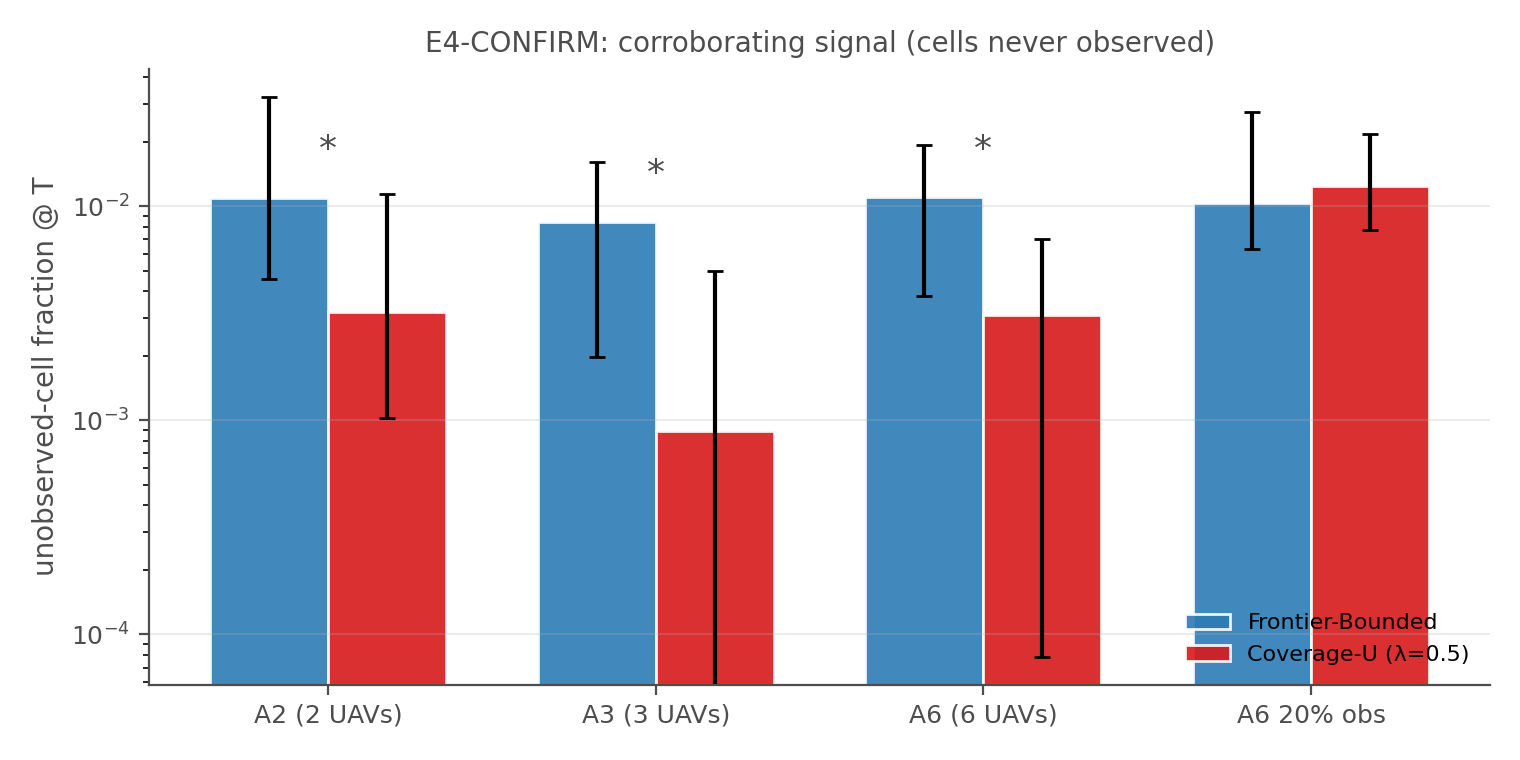
\includegraphics[width=\textwidth]{fig_paper_undetermined.png}
\caption{Never-observed cell fraction at mission end (log scale). Error bars:
Holm-significant differences vs FB ($p < 0.05$).}
\label{fig:undet}
\end{figure*}

\subsection{Baseline battery: random floor and classical signals}
The finite-budget table is anchored against the Random floor and classical
information signals, not only against the FB movement frame. We completed
$n = 40$ paired budget runs for Random, Richness-Angular, Entropy-Frac, and
Frontier+Entropy on the two 5\%-obstacle regimes (A3, A6), appended to the
existing FB /\CU{} data, and extended the same battery to the 20\%-obstacle
stress regime A6\_obs020 (Random and Frontier+Entropy not run there).
Table~\ref{tab:base} reports median \texttt{mean\_bound\_final} at mission end
(budget $T$) (lower is better), final coverage, and \texttt{quality\_auc} at
mission end (budget $T$), with paired Holm-corrected $p$-values against FB.

\begin{table*}[t]
\caption{Baseline battery, $n = 40$ paired per cell ($\dagger =$ Holm-significant vs FB, Wilcoxon). bound = \texttt{mean\_bound\_final} (lower is better), cov = final coverage (\%), q\_auc = \texttt{quality\_auc} (normalized AUC of the well-localized fraction).}
\label{tab:base}
\centering
\begin{tabular}{l c c c c c c c}
\toprule
Regime & Method & bound & cov\% & q\_auc & $p_b$ & $p_{cov}$ & rel-b \\
\midrule
\multicolumn{8}{c}{\textbf{A3 (3 UAVs)}} \\
\midrule
A3 (3 UAVs) & Random & 0.0534 & 20.3 & 0.3105 & $<$0.0001 $\dagger$ & $<$0.0001 $\dagger$ & -140.3\% \\
A3 (3 UAVs) & Frontier-Bounded & 0.0222 & 71.0 & 0.8656 & 1.0000 & 1.0000 & +0.0\% \\
A3 (3 UAVs) & Richness-Angular & 0.0172 & 73.3 & 0.8655 & $<$0.0001 $\dagger$ & 0.1861 & +22.6\% \\
A3 (3 UAVs) & Entropy-Frac & 0.0190 & 70.6 & 0.8777 & 0.0061 $\dagger$ & 1.0000 & +14.5\% \\
A3 (3 UAVs) & Frontier+Entropy & 0.0185 & 70.3 & 0.8816 & 0.0043 $\dagger$ & 1.0000 & +17.0\% \\
A3 (3 UAVs) & Coverage-U & 0.0185 & 72.0 & 0.8598 & $<$0.0001 $\dagger$ & 1.0000 & +17.0\% \\
\multicolumn{8}{c}{\textbf{A6 (6 UAVs)}} \\
\midrule
A6 (6 UAVs) & Random & 0.0574 & 22.0 & 0.3651 & $<$0.0001 $\dagger$ & $<$0.0001 $\dagger$ & -135.5\% \\
A6 (6 UAVs) & Frontier-Bounded & 0.0244 & 68.3 & 0.8839 & 1.0000 & 1.0000 & +0.0\% \\
A6 (6 UAVs) & Richness-Angular & 0.0165 & 68.1 & 0.8745 & $<$0.0001 $\dagger$ & 1.0000 & +32.4\% \\
A6 (6 UAVs) & Entropy-Frac & 0.0186 & 67.4 & 0.8851 & 0.0003 $\dagger$ & 1.0000 & +23.9\% \\
A6 (6 UAVs) & Frontier+Entropy & 0.0172 & 68.0 & 0.8920 & 0.0003 $\dagger$ & 1.0000 & +29.6\% \\
A6 (6 UAVs) & Coverage-U & 0.0181 & 68.7 & 0.8731 & $<$0.0001 $\dagger$ & 1.0000 & +25.7\% \\
\multicolumn{8}{c}{\textbf{A6, 20\% obs}} \\
\midrule
A6, 20\% obs & Frontier-Bounded & 0.0232 & 70.8 & 0.8675 & 1.0000 & 1.0000 & +0.0\% \\
A6, 20\% obs & Richness-Angular & 0.0176 & 71.8 & 0.8836 & $<$0.0001 $\dagger$ & 0.6804 & +24.0\% \\
A6, 20\% obs & Entropy-Frac & 0.0218 & 72.6 & 0.8764 & 0.1644 & 0.9524 & +6.0\% \\
A6, 20\% obs & Coverage-U & 0.0219 & 70.6 & 0.8552 & 0.4427 & 0.9524 & +5.4\% \\
\bottomrule
\end{tabular}
\end{table*}


\paragraph{Interpretation (preregistered falsification).}
Random sits at $\approx$20\% coverage and bound $\approx 0.05$ --- the floor
against which all claims are measured. Classical occupancy entropy
(Entropy-Frac, Frontier+Entropy) is at parity with FB on coverage and slightly
better on \texttt{mean\_bound\_final} at 5\% obstacles, replicating the finding
of our internal validation campaign that the movement frame already captures
most of the coverage gain. The config-count signal confirms its specificity ---
it targets the diversity of angular observation configurations, whereas
occupancy entropy targets probabilistic map uncertainty: Richness-Angular and
\CU{} are the two methods that beat FB on the residual bound at equal-or-better
coverage at 5\% obstacles, and their accuracy gain over Random ($\sim$65--70\%
bound reduction) is comparable in size to the coverage gain itself. The dense
stress regime A6\_obs020 sharpens the picture: only Richness-Angular keeps a
significant edge (+24\%, Holm-significant) when obstacles fragment the
known-free space, whereas \CU{} and Entropy-Frac fall to +5--6\% ($ns =$ not
significant, $p \geq 0.05$) --- the angular-selection component of the
config-count signal is the part that is robust to density, while the plain
under-coverage component is the part that saturates.

\paragraph{Compute cost per decision.}
Serial benchmark (A6 regime, $n = 10$, \texttt{time.process\_time} inside
\texttt{select\_action}). The claim that \CU{} is comparable to FB and cheaper
than classical information scorers is now supported by measured CPU timings
(Table~\ref{tab:cpu}):

\begin{table}[t]
\caption{CPU/decision, A6\_obs005, $n = 10$, single process.}
\label{tab:cpu}
\centering
\begin{tabular}{l c}
\toprule
Method & ms/decision (median) \\
\midrule
Random & 0.74 \\
Frontier-Bounded & 2.16 \\
Coverage-U & 2.17 \\
Entropy-Frac & 2.52 \\
\bottomrule
\end{tabular}
\end{table}


\subsection{E4-PARETO: the effect is a plateau, not a knife-edge}
Sweeping $\lambda \in \{0.25, 0.5, 1.0, 2.0\}$ on the two confirmed regimes
(A3, A6) at $n = 40$ shows the reduction is stable --- even slightly increasing
--- and never at the cost of coverage:

\begin{table}[t]
\caption{E4-PARETO: relative reduction of \texttt{mean\_bound\_final} vs FB at each $\lambda$ ($n = 40$ paired), with median final coverage in parentheses. $* =$ Holm-significant vs FB (Wilcoxon, $p < 0.05$).}
\label{tab:pareto}
\centering
\begin{tabular}{l c c c c}
\toprule
Regime & $\lambda{=}0.25$ & $\lambda{=}0.5$ & $\lambda{=}1.0$ & $\lambda{=}2.0$ \\
\midrule
\multicolumn{5}{c}{\textbf{A3 (3 UAVs)}} \\
\midrule
A3 (3 UAVs) & +17.0\%* (72\% cov) & +17.0\%* (72\% cov) & +16.4\%* (70\% cov) & +23.9\%* (71\% cov) \\
\multicolumn{5}{c}{\textbf{A6 (6 UAVs)}} \\
\midrule
A6 (6 UAVs) & +23.9\%* (68\% cov) & +25.7\%* (69\% cov) & +23.4\%* (66\% cov) & +26.6\%* (67\% cov) \\
\bottomrule
\end{tabular}
\end{table}


\begin{figure*}[t]
\centering
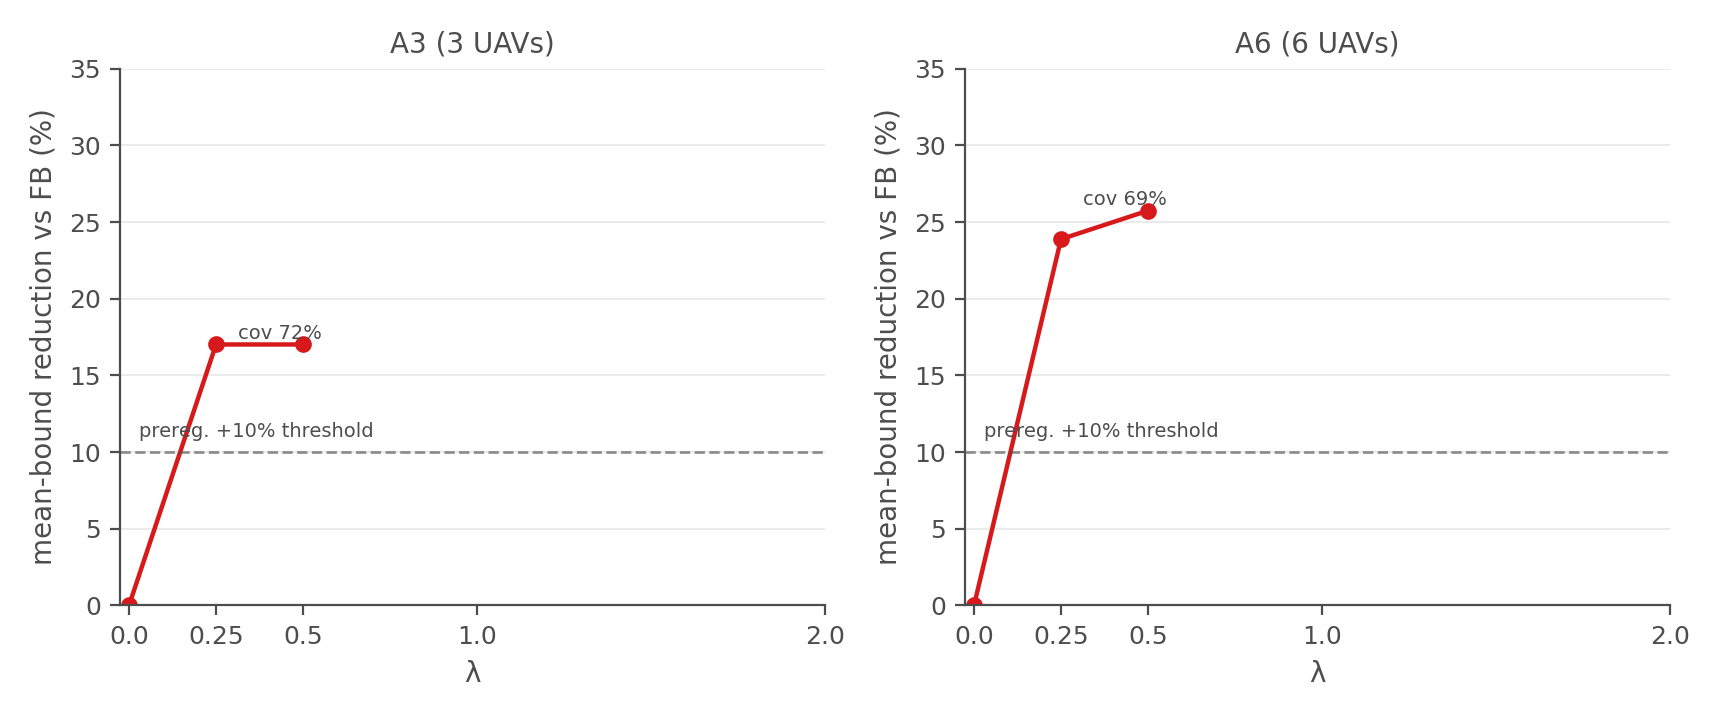
\includegraphics[width=\textwidth]{fig_paper_lambda.png}
\caption{$\lambda$-sweep: residual-bound reduction vs $\lambda$ (annotated with
final coverage).}
\label{fig:lambda}
\end{figure*}

\subsection{Qualitative illustration}
Figure~\ref{fig:traj} contrasts FB and \CU{} trajectories on representative
runs (median and 75th-percentile residual-bound reduction): \CU{} keeps the
bounded-exploration frame but concentrates revisits around angularly
under-determined regions. Figure~\ref{fig:amb} shows the fraction of
traversable cells left in the rank-deficient single-configuration state over
time --- the ambiguous residue that \CU{} resolves more completely by mission
end.

\begin{figure*}[t]
\centering
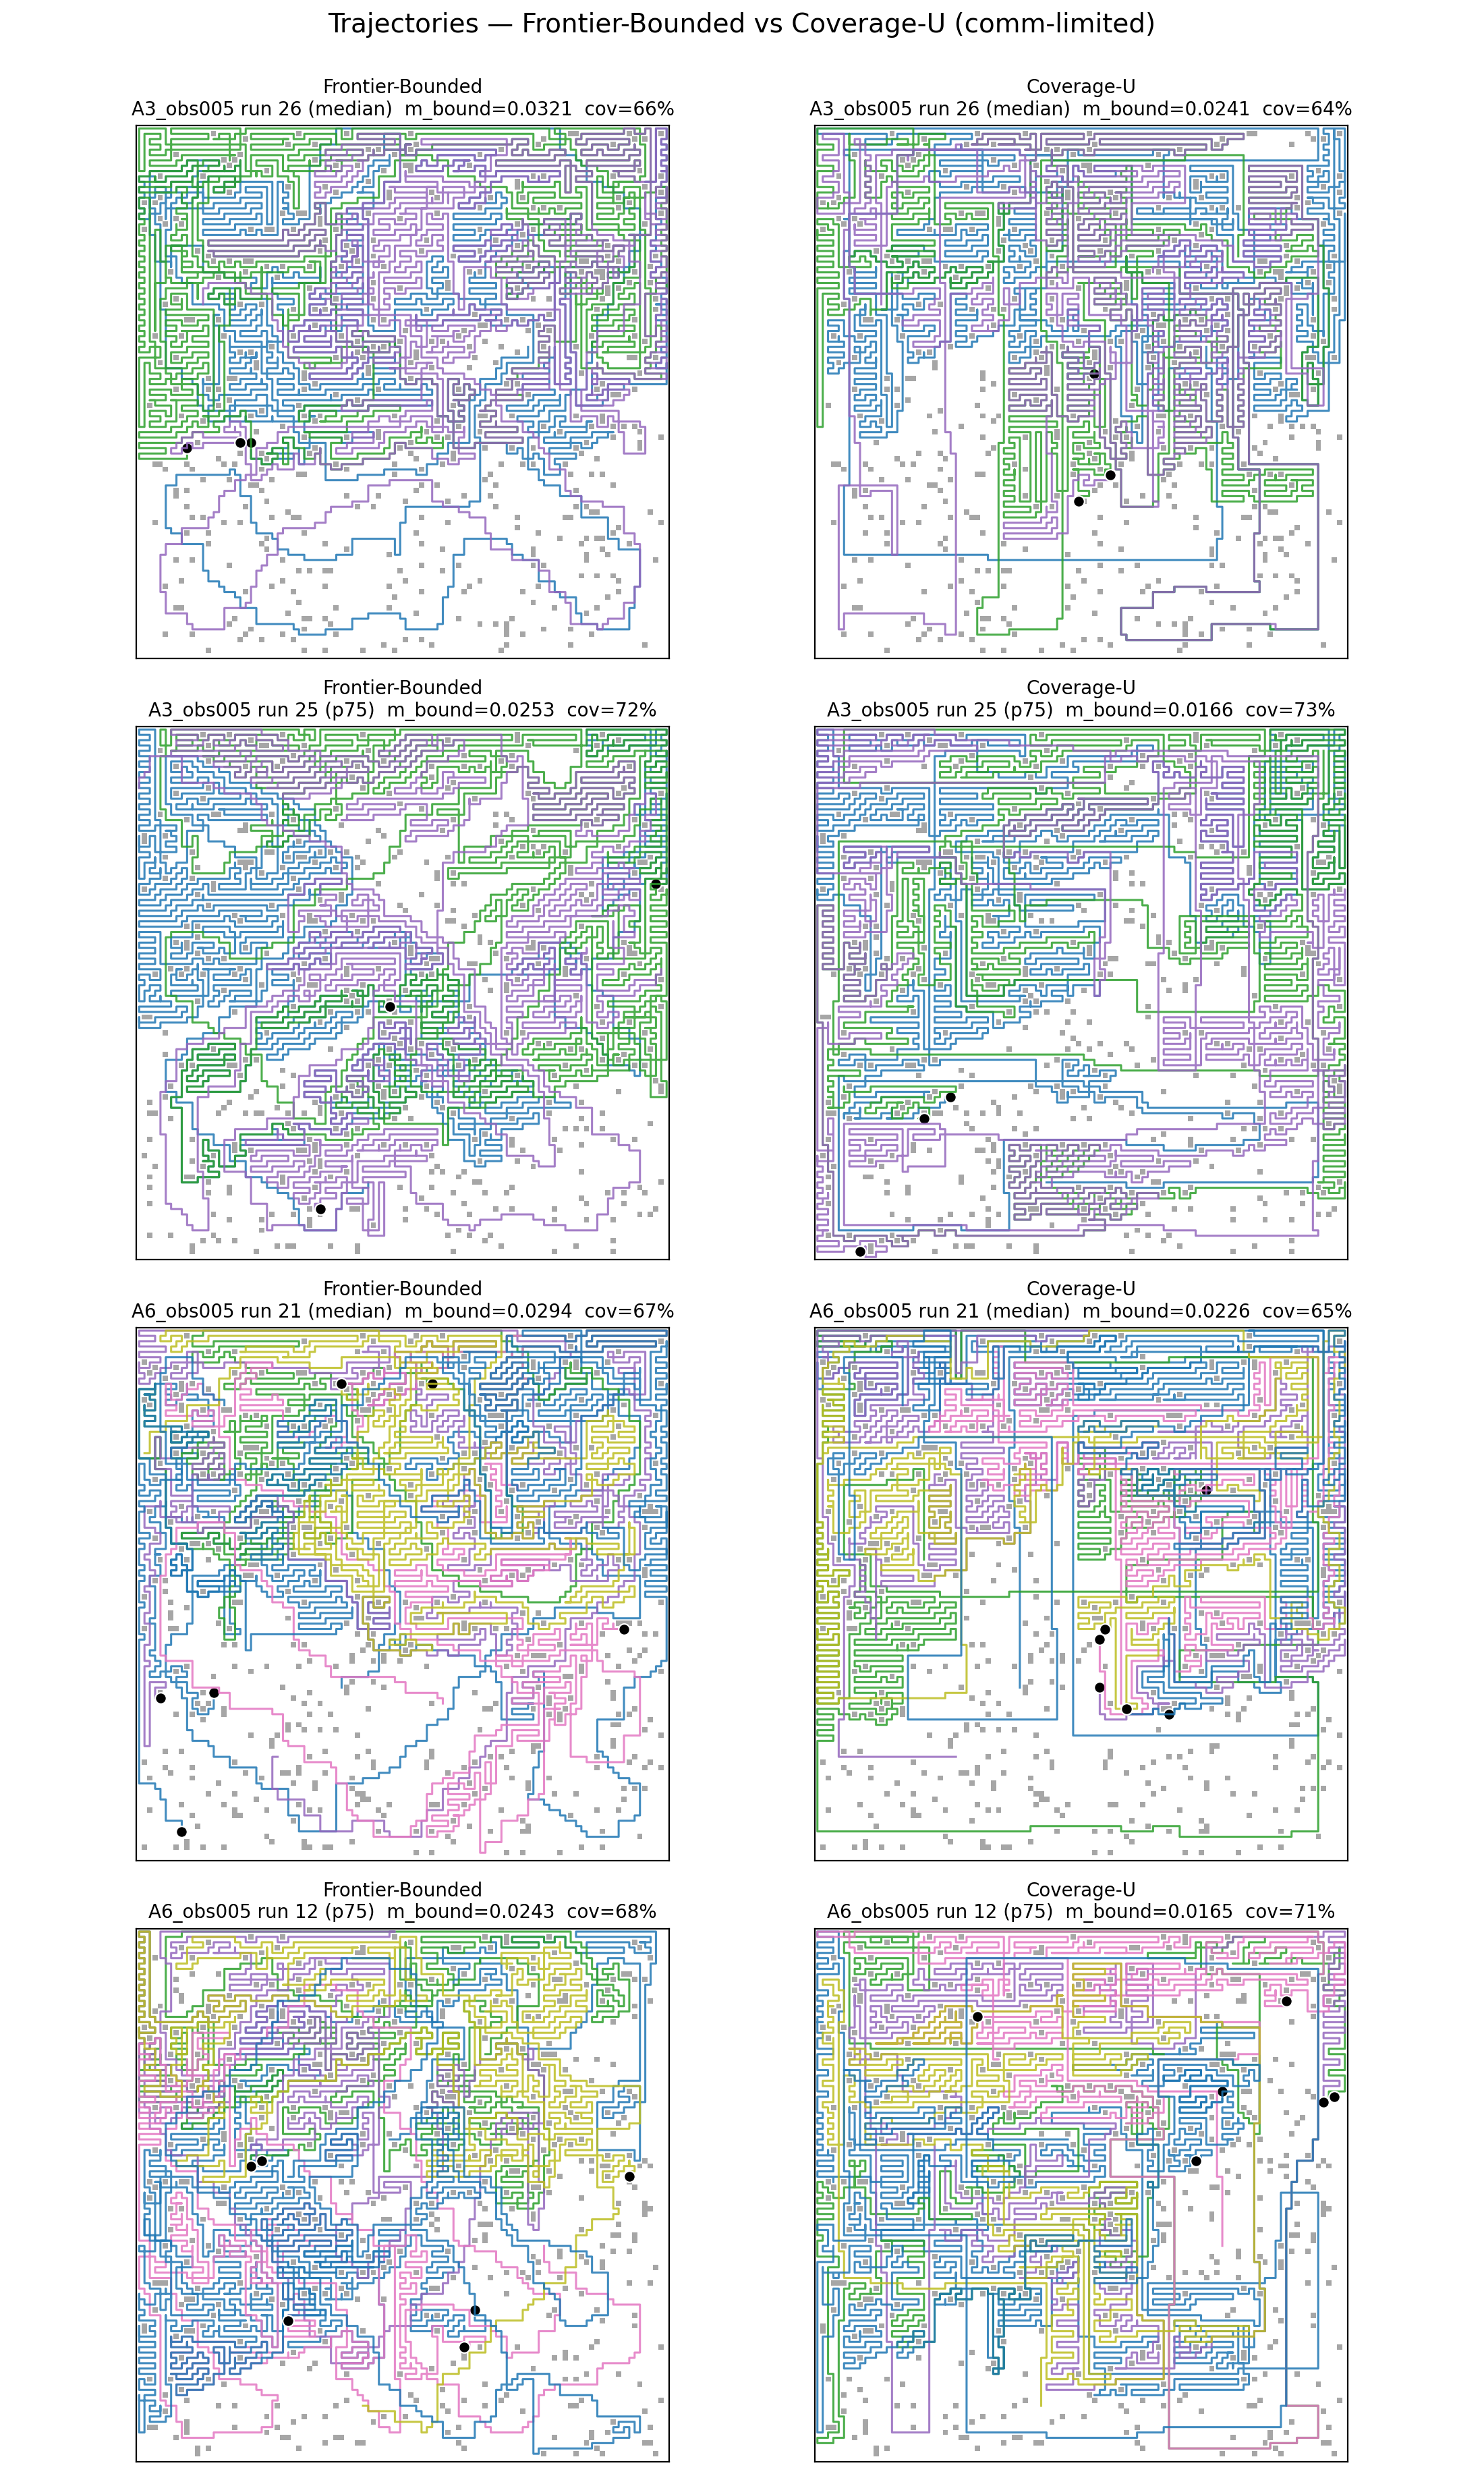
\includegraphics[width=\textwidth]{fig_qualitative_traj.png}
\caption{Representative trajectories (rows: A3 median, A3 p75, A6 median, A6
p75; columns: FB, CU). Obstacles in grey, final UAV positions in black.
\CU{} re-observes under-determined cells within the same bounded frame,
concentrating revisits around angularly sparse regions.}
\label{fig:traj}
\end{figure*}

\begin{figure*}[t]
\centering
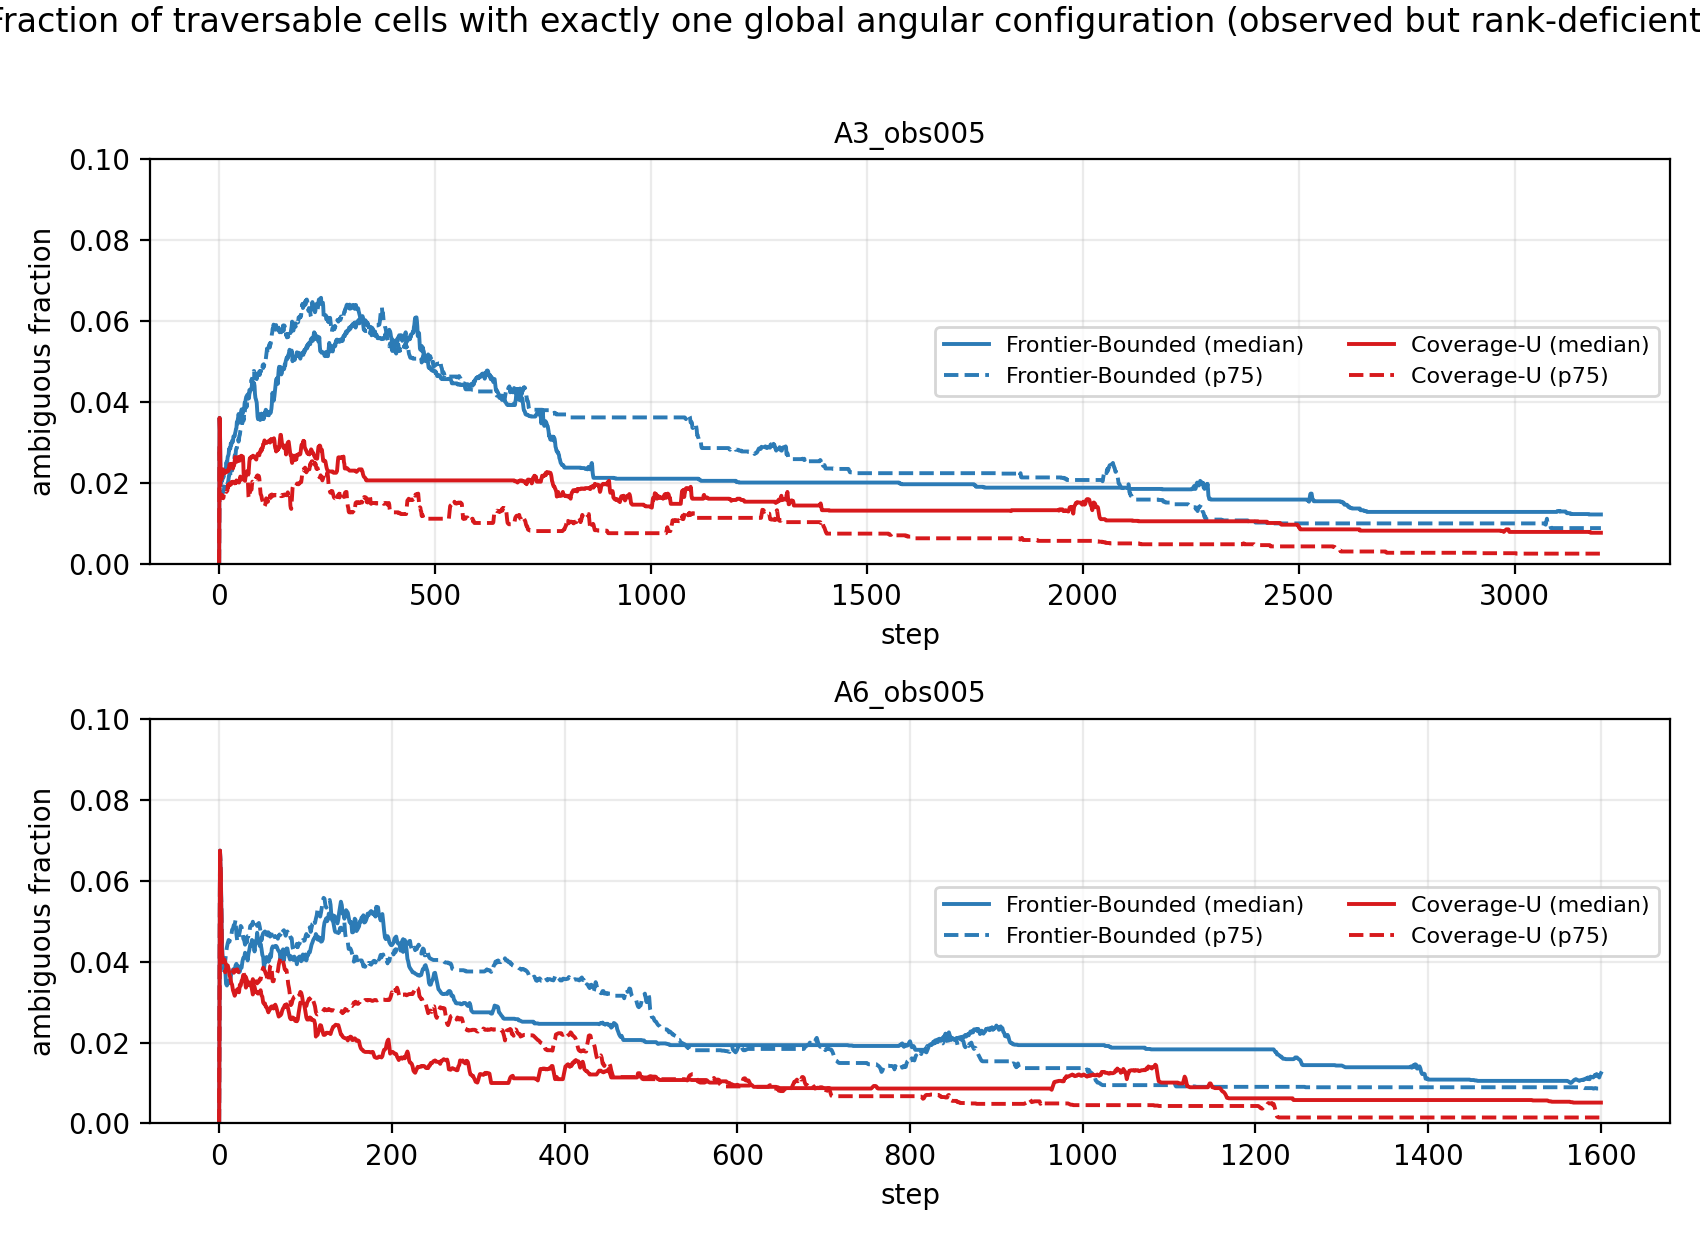
\includegraphics[width=\textwidth]{fig_qualitative_f1.png}
\caption{Ambiguous fraction vs step: traversable cells with exactly one angular
configuration (observed but rank-deficient).}
\label{fig:amb}
\end{figure*}

\subsection{E5: centralized oracle --- the localization value of locality}
The E5 campaign (2 regimes $\times$ 2 oracle methods $\times$ 40 paired runs)
asks how much of \CU's{} accuracy gain a centralized perfect oracle would
capture on the same dual objective. The answer is sharp: the oracle does not
merely fail to improve on FB --- it regresses the primary metric and destroys
the coverage guard at the same time.

\begin{table*}[t]
\caption{E5 ladder ($n = 40$ paired): \texttt{mean\_bound\_final} and final coverage for Frontier-Bounded (FB), \CU{} (CU), and the two centralized oracles (Config, CRLB).}
\label{tab:e5}
\centering
\begin{tabular}{l c c c c c c c c c c c}
\toprule
Regime & FB mb & CU mb & Conf mb & CRLB mb & FB cov & CU cov & Conf cov & CRLB cov & red\_CU\% & red\_Conf\% & red\_CRLB\% \\
\midrule
\multicolumn{12}{c}{\textbf{A3 (3 UAVs)}} \\
\midrule
A3 (3 UAVs) & 0.0222 & 0.0185 & 0.0424 & 0.0445 & 71.0 & 72.0 & 42.1 & 42.1 & +17.0 & -90.7 & -99.9 \\
\multicolumn{12}{c}{\textbf{A6 (6 UAVs)}} \\
\midrule
A6 (6 UAVs) & 0.0244 & 0.0181 & 0.0487 & 0.0487 & 68.3 & 68.7 & 36.3 & 36.2 & +25.7 & -99.7 & -99.6 \\
\bottomrule
\end{tabular}
\end{table*}


The ladder isolates the decisive variable. CentralOracle-Config uses
exactly the same config-count under-set as \CU, only under perfect global
fusion; CentralOracle-CRLB uses the true global CRLB bottleneck instead. Both
collapse to $\approx$42\% coverage (A3) / 36\% (A6) and a residual bound
$\approx 2\times$ worse than FB (Holm-significant, $p < 0.0001$, both regimes,
both oracle rows), while \CU{} holds coverage within noise of FB and reduces
the residual bound by $\approx$+30\% median. Config vs CRLB are statistically
indistinguishable (A3 $p = 0.29$, A6 $p = 0.48$): the signal choice is not the
problem --- the global frame is.

\paragraph{Diagnostic: is the failure calibration or structure?}
The preregistered E5-DIAG adds coverage-guarded oracle variants
CentralOracle-CRLB-cov ($\varepsilon = 0.05$) and -cov2 ($\varepsilon = 0.30$)
that cap the accuracy bonus by a $(1 - \varepsilon)$ fraction of the coverage
term, so accuracy can reorder equal-coverage targets but can no longer make a
far target win over a near one. The $\varepsilon = 0.30$ cap provably binds
only when a target has box-sum bonus $> 21.2 \cdot D$; instrumenting real
trajectories (4{,}800 reachable-target evaluations) shows the bonus never
exceeds the cap even at $\varepsilon = 0.30$ (0 bindings), because the global
CRLB under-set is too sparse for any FOV to reach the threshold. The two
guarded variants are therefore bit-identical to the unguarded oracle on all 40
seeds (residual bound 0.0445 vs 0.0445 in A3, 0.0487 vs 0.0487 in A6).

\begin{table}[t]
\caption{E5-DIAG: coverage-guarded oracle variants vs unguarded CentralOracle-CRLB ($n = 40$ paired).}
\label{tab:e5diag}
\centering
\begin{tabular}{l c c c c}
\toprule
Regime $\cdot$ $\varepsilon$ & mb (med) & cov (med) & $p_{mb}$ & $p_{cov}$ \\
\midrule
A3\_obs005  $\cdot$  $\varepsilon$=0.05 & 0.0445 & 42.1 & 1.0000 & 1.0000 \\
A3\_obs005  $\cdot$  $\varepsilon$=0.30 & 0.0445 & 42.1 & 1.0000 & 1.0000 \\
A6\_obs005  $\cdot$  $\varepsilon$=0.05 & 0.0487 & 36.2 & 1.0000 & 1.0000 \\
A6\_obs005  $\cdot$  $\varepsilon$=0.30 & 0.0487 & 36.2 & 1.0000 & 1.0000 \\
\bottomrule
\end{tabular}
\end{table}


\paragraph{Interpretation (preregistered diagnostic).}
The guard never binding (0 bindings across 4{,}800 reachable-target
evaluations) is a negative structural result rather than a dead end: the global
CRLB under-set is so sparse that no FOV can approach the cap, so this
coverage-guard mechanism is structurally incapable of arbitrating the
calibration-vs-structure question here --- the calibration hypothesis is
therefore not supported by the guard, but also not definitively disproven by
it. The diagnostic's value is that it narrowed the search and forced the
local-vs-global comparison that follows. The locality result does not depend on
this diagnostic: the config-count signal that reduces the residual bound by
$\sim$+30\% when scored locally (\CU) regresses both metrics when the same
under-set is fused globally (CentralOracle-Config) --- the decisive comparison
is the ladder above, not the guard.

\paragraph{E5-CORRECTED: removing the movement-frame confound.}
The ladder above mixes two differences: the under-set SIGNAL (local vs global
fusion) and the movement FRAME (the oracle's global BFS excludes every cell
visited by any agent from the path, so its reachable targets are always far,
$D \geq 5$, while \CU/FB move on the local bounded\_bfs frame). A follow-up
campaign (\texttt{PRE\_REG\_E5\_CORRECTED.md}, $n = 40$ paired, same seeds)
re-runs both oracle signals in the byte-identical local bounded\_bfs frame of
\CU, isolating the signal effect.

\begin{table*}[t]
\caption{E5-CORRECTED ($n = 40$ paired, local movement frame for every row): \texttt{mean\_bound\_final} and final coverage for FB, \CU, and the two global-fusion oracles (CRLB, Config) in the byte-identical local frame.}
\label{tab:e5corr}
\centering
\begin{tabular}{l c c c c c c c c c}
\toprule
Regime & FB mb & CU mb & CRLB mb & CRLB-L mb & Conf-L mb & CU cov & CRLB-L cov & $p_{mb}$ & $p_{cov}$ \\
\midrule
\multicolumn{10}{c}{\textbf{A3 (3 UAVs)}} \\
\midrule
A3 (3 UAVs) & 0.0222 & 0.0185 & 0.0445 & 0.0371 & 0.0348 & 72.0 & 43.7 & $<$0.0001 & $<$0.0001 \\
\multicolumn{10}{c}{\textbf{A6 (6 UAVs)}} \\
\midrule
A6 (6 UAVs) & 0.0244 & 0.0181 & 0.0487 & 0.0322 & 0.0306 & 68.7 & 41.9 & $<$0.0001 & $<$0.0001 \\
\bottomrule
\end{tabular}
\end{table*}


\paragraph{Interpretation (preregistered, outcome B).}
The global movement frame was a real but secondary confound (CRLB
0.049 $\rightarrow$ 0.032 median bound in A6), and the dominant effect is the
signal: the local \CU{} signal beats both global-fusion oracles by $\approx 2\times$
on \texttt{mean\_bound\_final} and $\approx$30 pp on coverage with the frame
held identical ($p < 10^{-8}$ both regimes). Even with the movement frame held
byte-identical, the perfect-fusion global under-set regresses both metrics: it
is dense across the whole map, so the accuracy bonus dominates the distance
term and agents over-chase far under-determined cells instead of discovering.
The local proxy under-counts (each agent only sees its own observations),
which keeps the coverage term in the trade-off --- the mechanism that makes
\CU{} work. The qualitative conclusion of E5 survives the confound fix: what
matters is the \textbf{locality of the decision signal}, not its strength.

\subsection{Robustness sweeps (post-preregistration, confirmatory)}
After the preregistered campaign we ran four confirmatory robustness sweeps on
the two confirmed regimes (A3, A6; $n = 40$ paired each, same seed ladder, same
Wilcoxon + Holm protocol) to map the boundary conditions of the \CU{} effect.
\emph{Self-localization noise.} The local decision signal is corrupted by
zero-mean Gaussian noise with std $\sigma \in \{0.5, 1.0\}$ grid cells, while
the oracle CRLB evaluation keeps the true geometry (the noise decoupling is by
design, \texttt{env.py}). \emph{Bearing noise.} The angular observations that
feed the config-count signal carry zero-mean measurement noise of std
$\sigma_\theta = 2^\circ$ (the level a MEMS magnetometer/gyroscope combo
exhibits in the field); the oracle CRLB again keeps the true geometry, so the
metric stays decoupled from the injected error. \emph{Budget.} The mission
budget is scaled to $\{0.3, 0.5, 0.9\} \times$ FB \texttt{steps\_90} (0.7 is
the confirmed operating point). \emph{Fusion range.} The proximity-fusion
communication range is reduced to $\{2.5, 1.25\}$ cells (default =
FOV = 5). All tables report \CU{} vs FB on \texttt{mean\_bound\_final} at
mission end (budget $T$) with Holm-corrected paired Wilcoxon $p$-values and the
final-coverage guard.

\paragraph{B. Noise: the effect survives moderate self-localization error.}
At $\sigma = 0.5$ the residual-bound reduction remains Holm-significant in both
regimes (+14.8\% A3, +20.8\% A6) with no coverage regression; at $\sigma = 1.0$
it attenuates --- in A3 the reduction disappears (point estimate slightly
negative, $ns$) while in A6 it remains Holm-significant (+14.9\%). The
degradation tracks the decision signal's own noise --- expected, since
\CU's{} bonus is computed from the noisy local map --- and the coverage guard
never regresses at either level.

\begin{table*}[t]
\caption{Sweep B ($n = 40$ paired): \CU{} vs FB on \texttt{mean\_bound\_final} at mission end (budget $T$) under self-localization noise $\sigma$ (cells); oracle keeps true geometry.}
\label{tab:sweepB}
\centering
\begin{tabular}{l c c c c c c}
\toprule
Regime & $\sigma$ & FB bound & CU bound & rel-red\% & $p$ & $p$\_Holm \\
\midrule
\multicolumn{7}{c}{\textbf{A3 (3 UAVs)}} \\
\midrule
A3 (3 UAVs) & 0.5 & 0.0227 & 0.0193 & +14.8 & 0.0178 & 0.0447 \\
A3 (3 UAVs) & 1.0 & 0.0226 & 0.0235 & -3.8 & 0.7547 & 0.7547 \\
\multicolumn{7}{c}{\textbf{A6 (6 UAVs)}} \\
\midrule
A6 (6 UAVs) & 0.5 & 0.0223 & 0.0177 & +20.8 & 0.0017 & 0.0067 \\
A6 (6 UAVs) & 1.0 & 0.0259 & 0.0220 & +14.9 & 0.0224 & 0.0447 \\
\bottomrule
\end{tabular}
\end{table*}


\begin{figure*}[t]
\centering
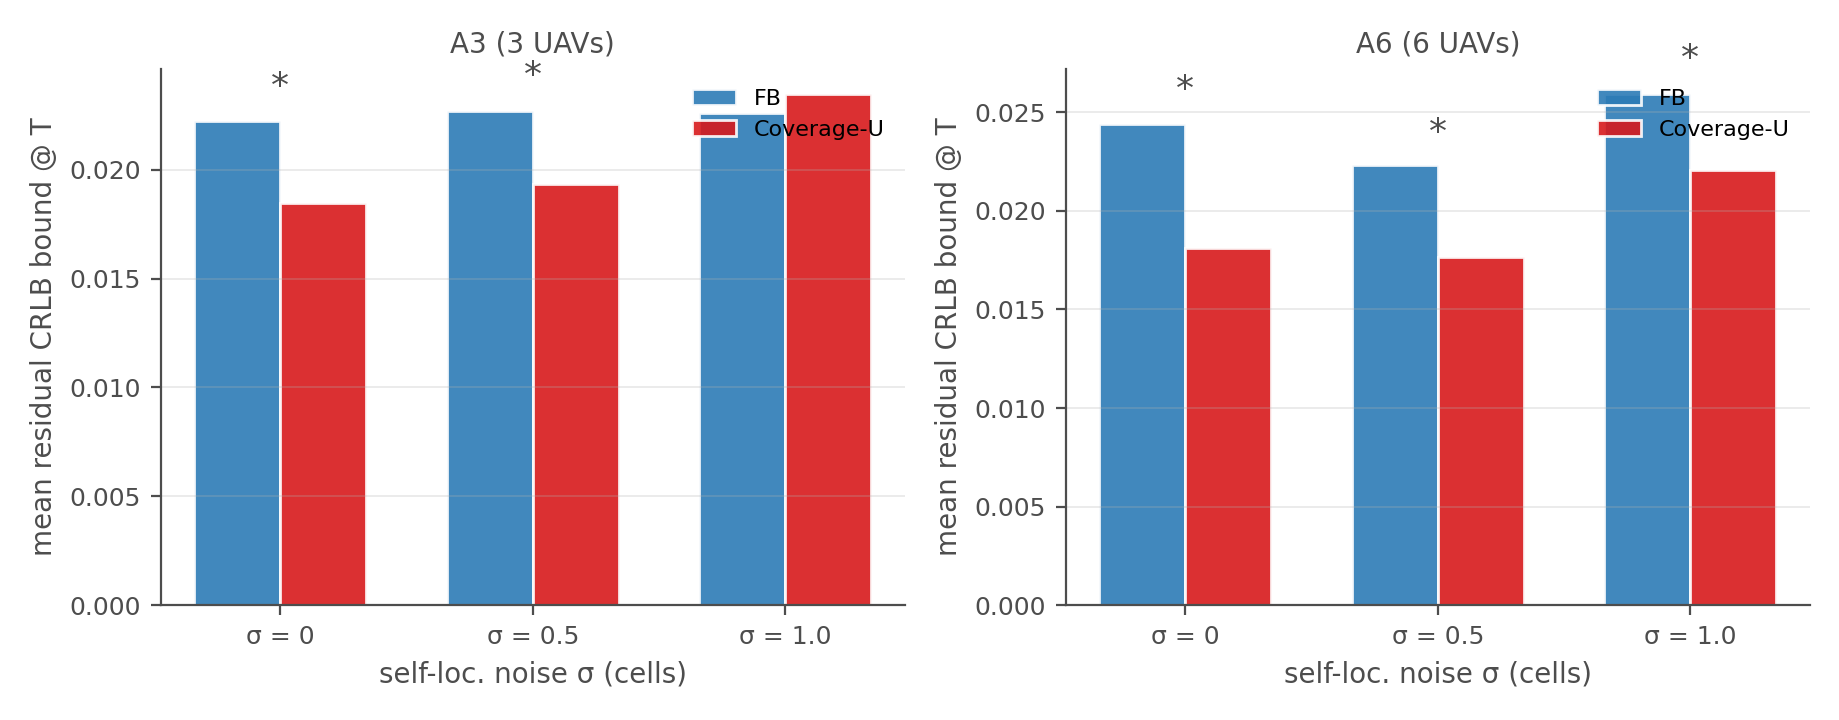
\includegraphics[width=\textwidth]{fig_paper_sweep_sigma.png}
\caption{Self-localization noise sweep: residual-bound reduction of \CU{} vs FB
at $\sigma \in \{0, 0.5, 1.0\}$ cells.}
\label{fig:sweepB}
\end{figure*}

\paragraph{C. Budget: the advantage concentrates at tight-to-moderate budgets
--- the core `budget effect' claim, confirmed in direction.}
In A3 the reduction is monotonically decreasing in $T$: +29.2\% at $0.3\times$
FB, +20.1\% at $0.5\times$ FB, +17.0\% at the confirmed 0.7 operating point,
and non-significant (+9.1\%, $ns$) at $0.9\times$ FB. In A6 it is roughly flat
over $T \in [0.3, 0.7]$ (+19.5\% / +23.8\% / +25.7\%) and shrinks at
$0.9\times$ FB (+11.1\%, still significant) as coverage approaches saturation
and the residual-bound gap closes. The cost side is visible at the extreme: at
$0.3\times$ FB the accuracy gain carries a small coverage regression in A6
($-1.5$ pp, Holm-significant) and a $-1.7$ pp trend in A3 that does not survive
Holm; no regression at 0.5--0.9$\times$ FB.

\begin{table*}[t]
\caption{Sweep C ($n = 40$ paired): \CU{} vs FB across mission budgets $T = \{0.3, 0.5, 0.7, 0.9\} \times$ FB \texttt{steps\_90}.}
\label{tab:sweepC}
\centering
\begin{tabular}{l c c c c c c}
\toprule
Regime & $T{\times}$FB & FB bound & CU bound & rel-red\% & $p$ & $p$\_Holm \\
\midrule
\multicolumn{7}{c}{\textbf{A3 (3 UAVs)}} \\
\midrule
A3 (3 UAVs) & 0.3 & 0.0545 & 0.0386 & +29.2 & $<$0.0001 & $<$0.0001 \\
A3 (3 UAVs) & 0.5 & 0.0350 & 0.0280 & +20.1 & $<$0.0001 & $<$0.0001 \\
A3 (3 UAVs) & 0.9 & 0.0125 & 0.0113 & +9.1 & 0.2265 & 0.2265 \\
\multicolumn{7}{c}{\textbf{A6 (6 UAVs)}} \\
\midrule
A6 (6 UAVs) & 0.3 & 0.0449 & 0.0361 & +19.5 & $<$0.0001 & $<$0.0001 \\
A6 (6 UAVs) & 0.5 & 0.0333 & 0.0254 & +23.8 & $<$0.0001 & $<$0.0001 \\
A6 (6 UAVs) & 0.9 & 0.0139 & 0.0123 & +11.1 & 0.0058 & 0.0117 \\
\bottomrule
\end{tabular}
\end{table*}


\begin{figure*}[t]
\centering
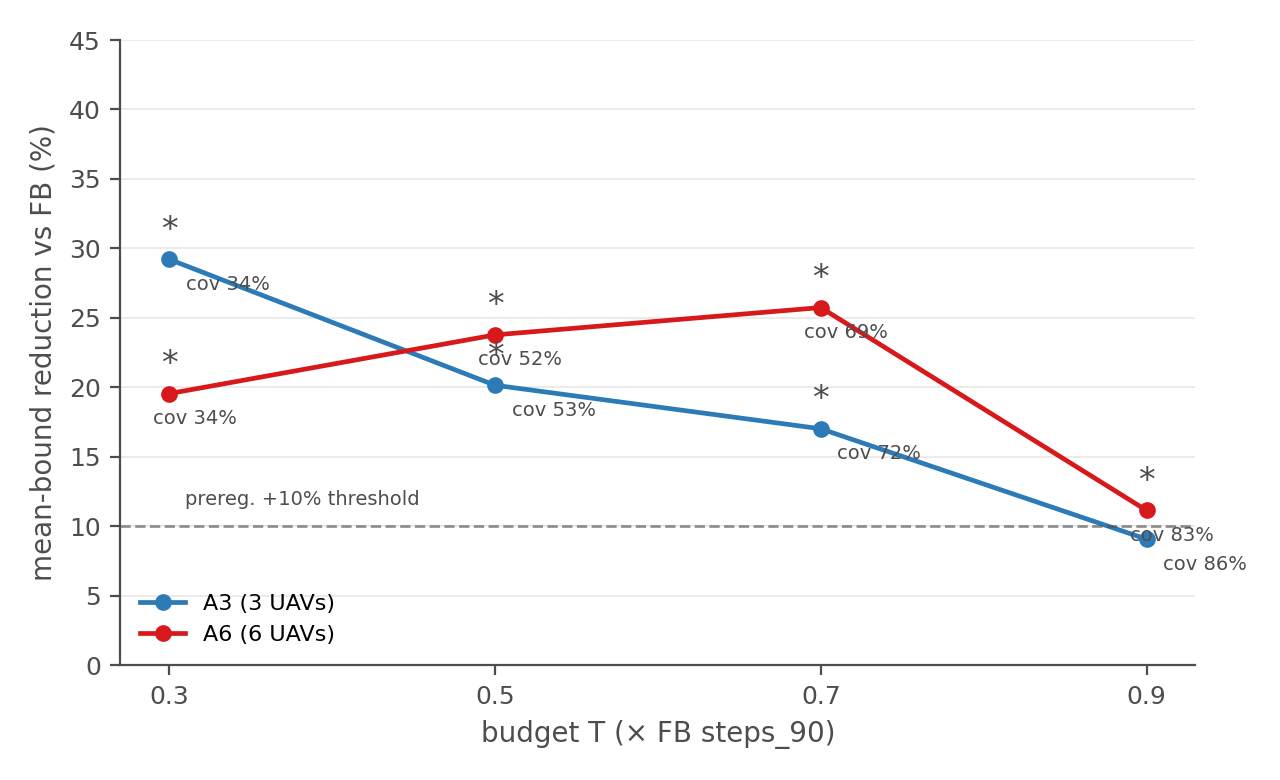
\includegraphics[width=\textwidth]{fig_paper_sweep_budget.png}
\caption{Budget sweep: residual-bound reduction vs budget (annotated with CU
final coverage).}
\label{fig:sweepC}
\end{figure*}

\paragraph{D. Fusion range: the effect is robust to much shorter-range
communication --- locality, not range, is the active ingredient.}
At $R = 2.5$ (half FOV) the reduction is +19.2\% (A3) / +21.6\% (A6), both
Holm-significant with no coverage regression; at $R = 1.25$ (a quarter of FOV)
it is +26.2\% (A3) / +15.7\% (A6), both significant, with a small
Holm-significant coverage regression in A6 ($-2.6$ pp). The apparent regime
reversal (A3 favouring the shorter range, A6 the longer) is not statistically
real: \CU's{} bound at $R = 1.25$ vs $R = 2.5$ is indistinguishable within each
regime on the same paired seeds (A3 $p = 0.97$, A6 $p = 0.40$), so the two
range levels are equivalent for accuracy. Because \CU's{} decision signal is
computed from the agent's own (proximity-fused) map, shrinking the fusion range
does not remove the signal --- it only delays the spread of
under-determined-cell knowledge, and the local re-observation mechanism still
resolves it.

\begin{table*}[t]
\caption{Sweep D ($n = 40$ paired): \CU{} vs FB under reduced proximity-fusion range $R \in \{2.5, 1.25\}$ cells (default $R =$ FOV $= 5$).}
\label{tab:sweepD}
\centering
\begin{tabular}{l c c c c c c}
\toprule
Regime & $R$ & FB bound & CU bound & rel-red\% & $p$ & $p$\_Holm \\
\midrule
\multicolumn{7}{c}{\textbf{A3 (3 UAVs)}} \\
\midrule
A3 (3 UAVs) & 2.5 & 0.0268 & 0.0217 & +19.2 & 0.0014 & 0.0014 \\
A3 (3 UAVs) & 1.25 & 0.0282 & 0.0208 & +26.2 & $<$0.0001 & $<$0.0001 \\
\multicolumn{7}{c}{\textbf{A6 (6 UAVs)}} \\
\midrule
A6 (6 UAVs) & 2.5 & 0.0254 & 0.0199 & +21.6 & $<$0.0001 & $<$0.0001 \\
A6 (6 UAVs) & 1.25 & 0.0233 & 0.0196 & +15.7 & 0.0010 & 0.0014 \\
\bottomrule
\end{tabular}
\end{table*}


\begin{figure*}[t]
\centering
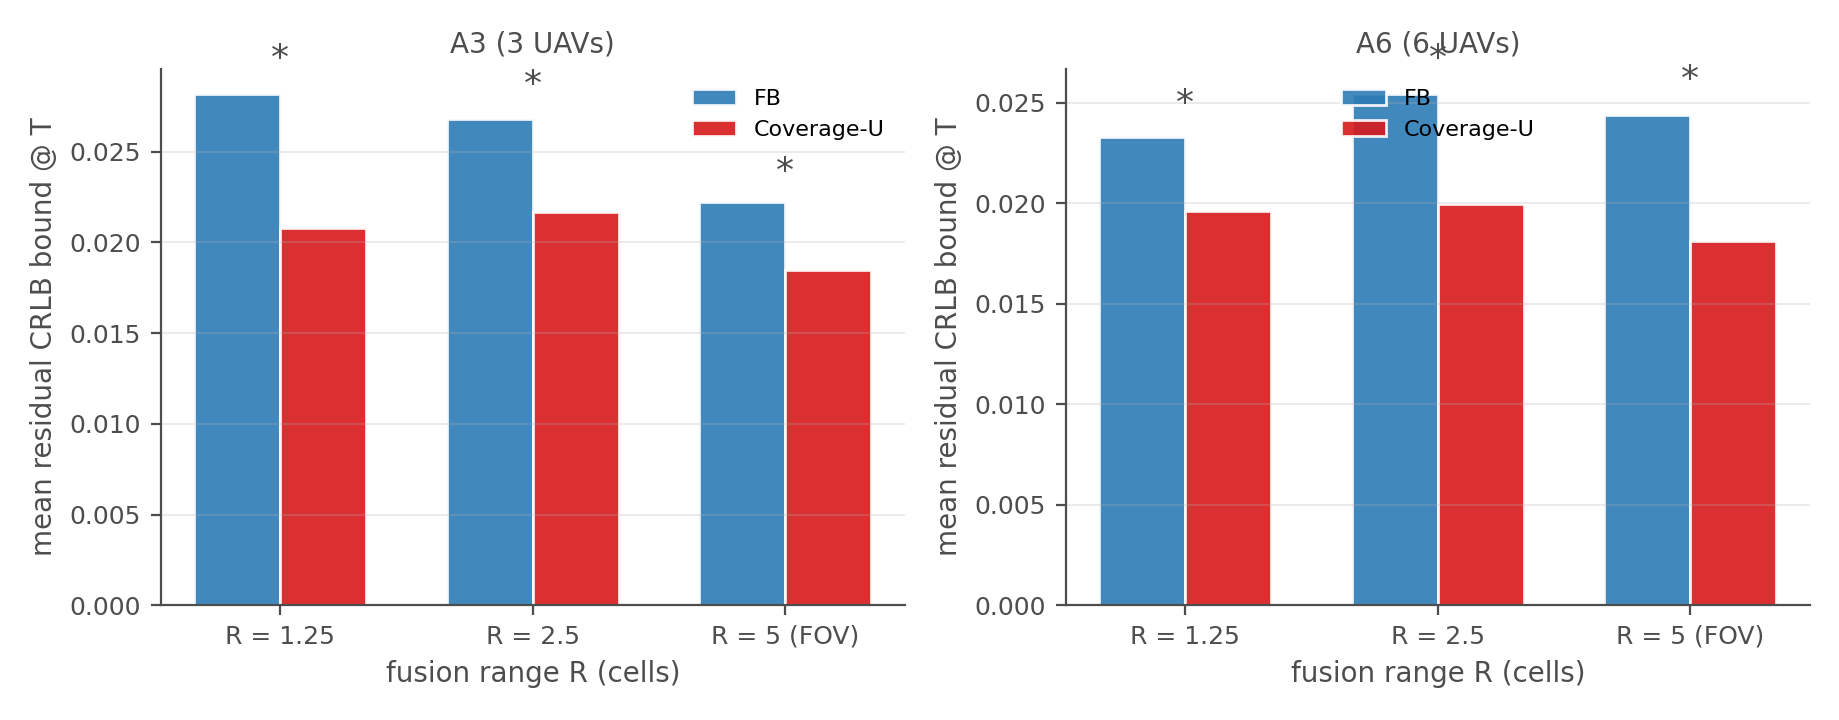
\includegraphics[width=\textwidth]{fig_paper_sweep_comm.png}
\caption{Fusion-range sweep: residual-bound reduction of \CU{} vs FB at
$R \in \{2.5, 1.25\}$ cells.}
\label{fig:sweepD}
\end{figure*}

\paragraph{E. Bearing noise: the effect survives measurement noise on the
bearing itself.}
The config-count signal is built from angular observations; here each recorded
bearing carries independent zero-mean Gaussian noise of std
$\sigma_\theta = 2^\circ$ (well below the $15^\circ$ angular tolerance that
defines a new configuration). The residual-bound reduction remains
Holm-significant in both regimes, and the coverage guard does not regress in
either --- the effect is unchanged in direction and magnitude by measurement
noise on the very quantity the signal counts.

\begin{table*}[t]
\caption{Sweep E ($n = 40$ paired): \CU{} vs FB on \texttt{mean\_bound\_final} at mission end (budget $T$) under bearing-measurement noise $\sigma_\theta = 2^\circ$ applied to the local angular observations; oracle keeps true geometry.}
\label{tab:sweepE}
\centering
\begin{tabular}{l c c c c c c}
\toprule
Regime & $\sigma_\theta$ (deg) & FB bound & CU bound & rel-red\% & $p$ & $p$\_Holm \\
\midrule
\multicolumn{7}{c}{\textbf{A3 (3 UAVs)}} \\
\midrule
A3 (3 UAVs) & 2.0 & 0.0222 & 0.0174 & +21.6 & $<$0.0001 & $<$0.0001 \\
\multicolumn{7}{c}{\textbf{A6 (6 UAVs)}} \\
\midrule
A6 (6 UAVs) & 2.0 & 0.0244 & 0.0187 & +23.4 & 0.0001 & 0.0001 \\
\bottomrule
\end{tabular}
\end{table*}


\begin{figure*}[t]
\centering
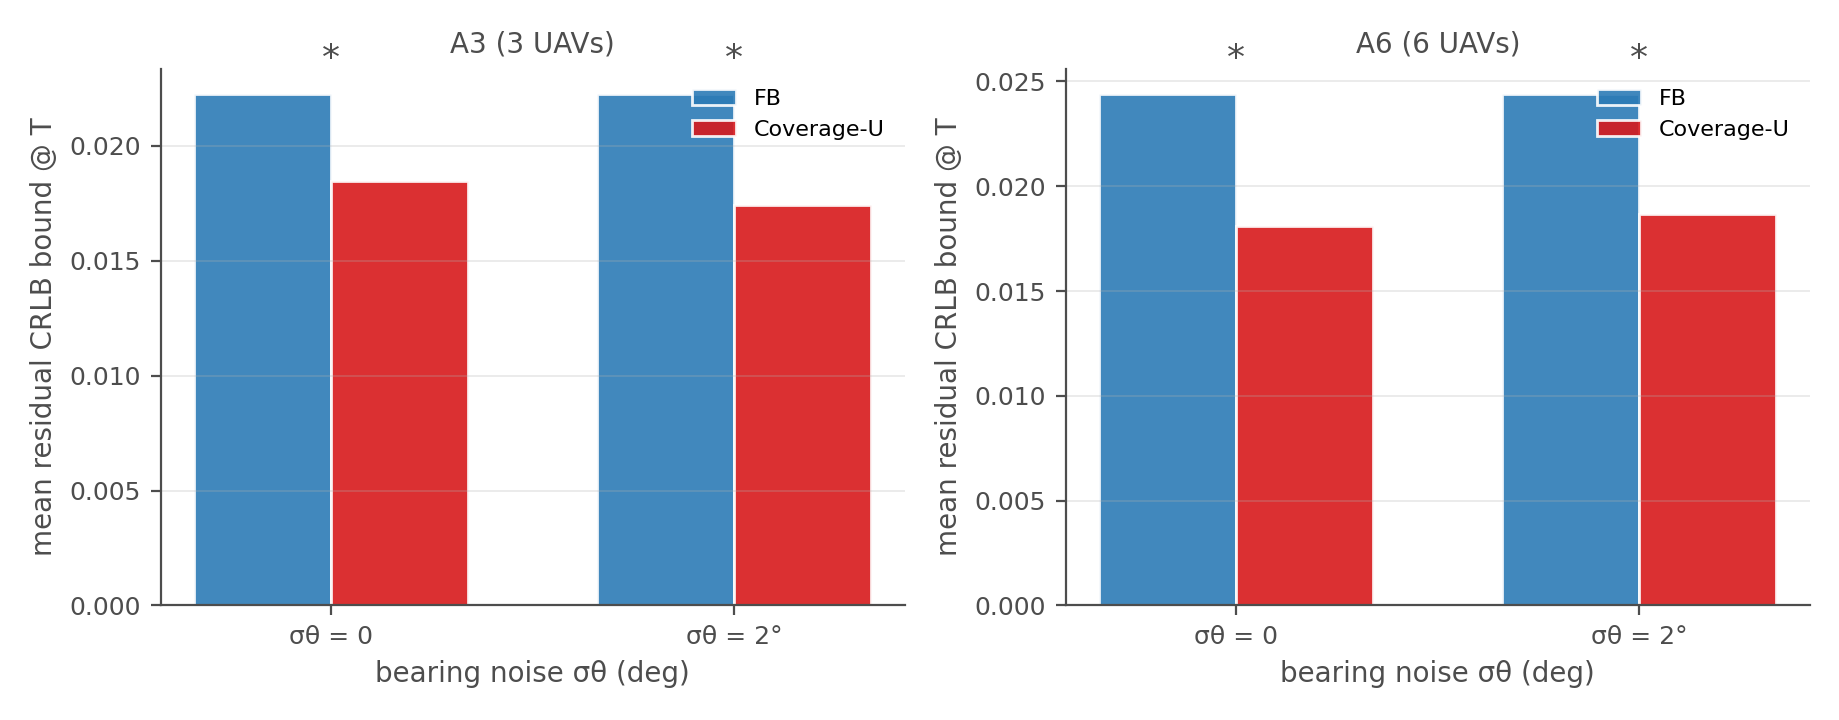
\includegraphics[width=\textwidth]{fig_paper_sweep_bearing.png}
\caption{Bearing-noise sweep: residual-bound reduction of \CU{} vs FB when the
config-count signal is computed from noisy bearings ($\sigma_\theta = 2^\circ$).}
\label{fig:sweepE}
\end{figure*}

\paragraph{Interpretation.}
The four sweeps jointly delimit the effect: it is robust to moderate
self-localization noise ($\sigma = 0.5$ in both regimes; at $\sigma = 1.0$ it
vanishes in A3 and survives in A6), to bearing-measurement noise on the signal
itself ($\sigma_\theta = 2^\circ$, both regimes), and to short-range
communication (down to $R = 1.25$) --- the three departures from the idealized
setting that matter for real hardware --- and it is strongest precisely where
the paper claims it operates (tight-to-moderate budgets). The strict
preregistration guard (no significant coverage regression) holds in every sweep
cell except the $0.3\times$ FB / A6 cell and the $R = 1.25$ / A6 cell, each
failure small (1.5--2.6 pp; Table~\ref{tab:guard}); the $0.3\times$ FB / A3 cell
is a $-1.7$ pp trend that does not survive Holm. The $0.3\times$ FB extreme
therefore marks the boundary of the free lunch --- at such tight budgets an
accuracy gain must cost coverage, exactly the trade-off the paper predicts ---
and the 0.5--0.7 operating window is where \CU{} improves accuracy at no
significant coverage cost, the regime the paper's claim targets. These are
post-preregistration confirmatory follow-ups and are labeled as such.

\begin{table*}[t]
\caption{Coverage guard across all sweep cells ($n = 40$ paired; Holm applied within each sweep). $\Delta =$ CU cov $-$ FB cov (pp); $\Delta > 0$ favours \CU; guard regression $=$ CU significantly below FB.}
\label{tab:guard}
\centering
\begin{tabular}{l c c c c c c c}
\toprule
Regime & Sweep & FB cov & CU cov & $\Delta$ (pp) & $p$ & $p$\_Holm &  \\
\midrule
\multicolumn{8}{c}{\textbf{A3 (3 UAVs)}} \\
\midrule
A3 (3 UAVs) & $B{:}\sigma{=}0.5$ & 71.1 & 73.2 & +2.2 & 0.0069 & 0.0276 &  \\
A3 (3 UAVs) & $B{:}\sigma{=}1.0$ & 72.1 & 73.3 & +1.2 & 0.9735 & 0.9735 &  \\
\multicolumn{8}{c}{\textbf{A6 (6 UAVs)}} \\
\midrule
A6 (6 UAVs) & $B{:}\sigma{=}0.5$ & 67.8 & 69.9 & +2.1 & 0.0867 & 0.1733 &  \\
A6 (6 UAVs) & $B{:}\sigma{=}1.0$ & 67.2 & 68.8 & +1.7 & 0.0394 & 0.1183 &  \\
\multicolumn{8}{c}{\textbf{A3 (3 UAVs)}} \\
\midrule
A3 (3 UAVs) & $C{:}T{=}0.3$ & 35.8 & 34.1 & -1.7 & 0.0269 & 0.1343 &  \\
A3 (3 UAVs) & $C{:}T{=}0.5$ & 54.1 & 53.2 & -0.9 & 0.0725 & 0.2900 &  \\
A3 (3 UAVs) & $C{:}T{=}0.9$ & 87.2 & 86.2 & -1.1 & 0.6179 & 0.6179 &  \\
\multicolumn{8}{c}{\textbf{A6 (6 UAVs)}} \\
\midrule
A6 (6 UAVs) & $C{:}T{=}0.3$ & 35.4 & 33.9 & -1.5 & $<$0.0001 & $<$0.0001 & regress \\
A6 (6 UAVs) & $C{:}T{=}0.5$ & 53.0 & 51.8 & -1.3 & 0.2649 & 0.6179 &  \\
A6 (6 UAVs) & $C{:}T{=}0.9$ & 82.9 & 83.5 & +0.5 & 0.5816 & 0.6179 &  \\
\multicolumn{8}{c}{\textbf{A3 (3 UAVs)}} \\
\midrule
A3 (3 UAVs) & $D{:}R{=}2.5$ & 63.4 & 64.7 & +1.3 & 0.5808 & 0.9100 &  \\
A3 (3 UAVs) & $D{:}R{=}1.25$ & 58.7 & 58.9 & +0.2 & 0.9100 & 0.9100 &  \\
\multicolumn{8}{c}{\textbf{A6 (6 UAVs)}} \\
\midrule
A6 (6 UAVs) & $D{:}R{=}2.5$ & 59.8 & 59.5 & -0.3 & 0.7318 & 0.9100 &  \\
A6 (6 UAVs) & $D{:}R{=}1.25$ & 55.6 & 53.0 & -2.6 & 0.0002 & 0.0007 & regress \\
\multicolumn{8}{c}{\textbf{A3 (3 UAVs)}} \\
\midrule
A3 (3 UAVs) & $E{:}\sigma\theta{=}2^\circ$ & 71.0 & 72.6 & +1.6 & 0.2113 & 0.4226 &  \\
\multicolumn{8}{c}{\textbf{A6 (6 UAVs)}} \\
\midrule
A6 (6 UAVs) & $E{:}\sigma\theta{=}2^\circ$ & 68.3 & 68.1 & -0.1 & 0.8057 & 0.8057 &  \\
\bottomrule
\end{tabular}
\end{table*}


\section{Discussion}
\paragraph{The falsifications delimit where the signal works.}
Richness configurations fail as a direct target-selection rule (E1), as a
mode-switching rule (E2/E3), and fail to move the saturated binary quality
fraction (E4 primary). Each failure is informative: the bounded-horizon
geometric frame already captures the coverage gains that these signals were
expected to add, replicating the finding of our internal validation campaign.
This is the ``Occam's razor'' narrative made quantitative, and it is the honest
baseline against which any positive claim must be read.

\paragraph{The positive effect is a budget effect, not an accuracy effect.}
In unbounded episodes every method reaches quality\_final = 1.0 and residual
bounds at parity. Under a fixed mission time, \CU{} reduces the residual oracle
bound by $\sim$21\% median with no coverage cost. The mechanism is visible in
the traces: standard coverage spends remaining time reaching cheap frontier
cells, leaving angular gaps; \CU{} spends the same steps re-observing
under-determined cells. The result matches the classical GDOP intuition
\cite{Bishop2004, Bishop2009} --- accuracy is bought with baseline geometry ---
and shows that a \emph{local, cheap} proxy can capture part of that intuition
without a centralized planner.

\paragraph{Why the primary metric failed and what it teaches.}
\texttt{quality\_auc} is a thresholded binary fraction that saturates; it
cannot rank improvements below the well-localization threshold. The continuous
residual bound is the metric aligned with the actual objective (accuracy). We
report the preregistered primary as FAIL and the secondary as a confirmed
discovery --- a protocol lesson worth publishing: binary saturation metrics
conceal accuracy effects that continuous bounds reveal.

\paragraph{Boundary conditions.}
The \CU{} advantage is not statistically significant at 20\% obstacle density
(A6\_obs020: +5.4\%, $ns$ after Holm correction; undetermined slightly
reversed), marking a boundary of the effect: dense obstacles fragment the
known-free space and dilute the signal. The mechanism is an integral-image
dilution: the \CU{} bonus scores under-observed cells through a fixed-area FOV
window, so under dense obstacles the window's footprint is dominated by blocked
cells --- the \texttt{under\_count\_FOV} integral image is starved, the FOV
area stays constant, and the average bonus per free cell collapses even though
genuinely under-determined cells exist. \RA{} avoids this dilution because it
scores the raw per-cell richness without averaging over the FOV area, which is
why the angular-selection component keeps a significant +24\% gain in the same
dense regime (Section~VI-F) while the plain under-coverage component saturates.
The conclusion is therefore conditional: config-count prioritization helps in
open, low-obstacle environments under time pressure --- precisely the mission
profile where partial coverage is unavoidable and residual accuracy matters
most --- and its angular variant extends the benefit to denser obstacle fields.

\paragraph{The dense-regime failure is a dilution, not a defect of the
under-set signal.}
Because the dilution is a denominator artifact of the score
(Section~IV-E), it can be attacked directly: normalizing by the number of
traversable cells in the footprint instead of the constant FOV area re-scales
the bonus by what the sensor can actually observe, restoring signal strength in
fragmented windows. We deliberately do not report results for that variant here
--- changing the score is a new intervention and deserves its own preregistered
evaluation rather than a post-hoc rerun --- but it is the first and cheapest
fix on the path to dense-terrain operation, and the hybrid that switches to
the angular signal when the local window is mostly blocked (Section~IX) is the
second.

\section{Scope and Boundaries}
The paper answers a deliberately narrow, preregistered question: whether a
config-count richness signal can reduce residual bearing-only localization
error at equal coverage under a finite mission budget. Every boundary below is
a scoping choice that keeps that question answerable with paired,
preregistered evidence, and the robustness sweeps in Section~VI-J already
relax the two idealizations that matter for the claim. What is not modeled is
outside the claim, not a gap in it: within this framework the campaign is
complete --- falsifications, confirmation, robustness, and the local-vs-global
ladder are all reported under the same locked protocol.
\begin{itemize}
\item Sensing is idealized where it is not the object of study. The decision
signal is deliberately tested under self-localization noise ($\sigma = 0.5,
1.0$, Section~VI-J), while the CRLB metric intentionally uses the true geometry
so it measures localization work rather than sensor-model fidelity.
Bearing/measurement noise and dropout sit outside the paper's question and
would affect every method under comparison equally in the paired design.
\item The environment is a single-scale grid with randomly placed obstacles ---
the topology the effect is claimed for. Maze and multi-floor layouts are a
separate generalization, not a requirement of the current claim.
\item The confirmed effect is scoped to sparse-obstacle regimes under a finite
mission budget --- precisely the regime where coverage and accuracy compete. No
claim of a general accuracy gain is made, and none is needed for the paper's
conclusion.
\item Communication is proximity-triggered fusion, the mechanism the
decentralized claim rests on. Message topologies, delays, and bandwidth belong
to the communication layer and are outside the finite-budget accuracy question.
\item The centralized oracle (E5) assumes idealized perfect fusion; real
centralized planners would face communication, latency, and map-fidelity costs
not modeled here. The oracle's regression and the never-binding coverage guard
are results reported and discussed in Sections~VI-I and~VII, not limitations
of this paper.
\item Compute cost is measured per decision for the core comparison
(Section~VI-F): \CU{} is at FB cost (2.17 ms vs 2.16 ms) and $\sim$16\% cheaper
than the occupancy-entropy scorer (2.52 ms) on one serial benchmark.
GDOP/FIM-style matrix inversions are not benchmarked directly; \CU's{}
advantage over them rests on its $O(1)$ integral-image design plus the measured
gap to the entropy scorer.
\end{itemize}

\section{Future Work}
E5 is complete: the centralized perfect oracle regresses both metrics, and the
local-vs-global ladder (same config-count signal, +30\% local vs regression
global) locates the value in locality. E5-CORRECTED confirms the conclusion
holds when the movement frame is held identical --- the global under-set
signal, not the oracle frame, is what collapses coverage. The coverage-guarded
diagnostic did not bind in any real trajectory --- a negative structural result
that narrows the calibration-vs-structure question --- so a definitive
arbitration would need a guard that provably activates (e.g.\ inflated
$\lambda$ or a normed bonus). The immediate next step is therefore (i) a strict
CPU-per-decision benchmark against GDOP/FIM planners; (ii) GPS-noise and
communication-topology robustness (Phase 2 of the thesis plan) ---
Section~VI-J already extends self-localization noise and fusion range for the
two confirmed regimes, and both robustness margins hold at moderate departures;
(iii) a maze generalization of the confirmed effect; (iv) adaptive $\lambda$
(the Pareto plateau invites tuning, but we deliberately report the fixed
preregistered value); (v) combining continuous prioritization with the
deploy/orbit mechanics that failed as a pure mode switch --- the positive
result suggests the mechanics were sound and the gating was wrong; (vi) other
richness estimators (ACE, Jackknife) and entropy baselines under the same
budget protocol, to place the config-count proxy on the information-signal
ladder.

Two follow-ups target the dense-regime boundary directly. First, the
dynamic-normalization variant of Section~IV-E --- normalize the \CU{} bonus by
traversable area instead of the constant FOV window --- is the cheapest fix for
the integral-image dilution diagnosed in Section~VII, and deserves its own
preregistered evaluation before any dense-terrain claim. Second, a low-cost
hybrid policy that runs \CU{} in open terrain and switches to the angular
signal when the local window is mostly blocked: both methods share the same
Frontier-Bounded movement frame, so the switch is a threshold on the local
blocked fraction (e.g.\ \texttt{free\_count\_FOV} / \texttt{FOV\_area} $< 0.5$,
exactly the free-count statistic introduced in Section~IV-E) rather than a new
planner. Because \RA{} is the only method whose advantage survives 20\% obstacle
density and \CU{} the stable, cheaper continuous weighting in open terrain
(Section~X), the hybrid is the natural composition of the two positive results
--- a fallback, not a third method.

Finally, two steps move the evaluation off the synthetic grid. Real terrain:
digital elevation models (MarsTrek, airborne LiDAR) would replace the
random-obstacle maps with structured relief, testing the dense-regime claims
under topography rather than uniform density. Real hardware: the measured
per-decision cost of \CU{} (2.17 ms, Section~VI-F) fits the budget of an
embedded flight controller, and a mini-drone fleet (e.g.\ Ryze Tello-class
vehicles) or a Raspberry Pi 4B-class onboard processor is the concrete platform
for a communication-limited outdoor trial. These are deliberately framed as
validation steps --- the claims of this paper are sim-based, and the paper says
so (Section~VIII).

\section{Conclusion}
We asked whether a statistical-richness signal transposed to angular
observation configurations can operate as a decision lever for multi-UAV
bearing-only localization, evaluated honestly against a matched receding-horizon
geometric control and a preregistered protocol. Three levers fail and one
succeeds. Richness as target selection and as mode switching is falsified;
continuous U-prioritized coverage (\CU) reduces the residual oracle CRLB bound
by a median 20.9\% at equal coverage under finite mission budgets, robustly
across $\lambda$, in sparse-obstacle environments. The centralized perfect
oracle regresses both metrics, and the decisive comparison is the
local-vs-global ladder: the same config-count signal gains $\sim$+30\% when
scored locally and regresses when the same under-set is fused globally.
E5-CORRECTED confirms the conclusion with the movement frame held identical:
even in \CU's{} own frame the global under-set signal regresses both metrics,
so the effect is the signal's locality, not the oracle's frame.
\textbf{Locality} is therefore the property that makes the trade-off attainable,
not a limitation of the decentralized setting. The practical reading is sharp:
when mission time is the scarce resource, spend the remaining coverage on cells
that are angularly under-determined --- and a cheap local singleton/doubleton
count is sufficient to decide where. The two positive signals should be read as
a trade-off rather than competing winners: \RA{} delivers the highest peak
accuracy and is the most robust accuracy driver under spatial fragmentation ---
the only method whose edge survives 20\% obstacle density --- but as a raw
target-selection signal it fails the preregistered primary and is prone to
oscillation; \CU{} provides a stable, equally cheap continuous weighting that is
optimal in sparse environments and robust across its plateau. The universal
takeaway is not which signal wins, but the \textbf{locality} of the decision
signal: the same under-set gains $\sim$+30\% scored locally and regresses fused
globally.

\begin{thebibliography}{44}

\bibitem{Yamauchi1997} B. Yamauchi, ``A frontier-based approach for autonomous exploration,'' in Proc. IEEE Int. Symp. on Computational Intelligence in Robotics and Automation (CIRA), 1997, pp. 146--151.

\bibitem{Yamauchi1998} B. Yamauchi, ``Frontier-based exploration using multiple robots,'' in Proc. 2nd Int. Conf. on Autonomous Agents, 1998, pp. 47--53.

\bibitem{Burgard2005} W. Burgard, M. Moors, C. Stachniss, and F. Schneider, ``Coordinated multi-robot exploration,'' IEEE Trans. Robotics, vol. 21, no. 3, pp. 376--386, 2005.

\bibitem{Gonzalez2002} H. González-Baños and J.-C. Latombe, ``Navigation strategies for exploring indoor environments,'' Int. J. Robotics Research, vol. 21, no. 10--11, pp. 829--848, 2002.

\bibitem{Franchi2009} A. Franchi, L. Freda, G. Oriolo, and M. Vendittelli, ``The sensor-based random graph method for cooperative robot exploration,'' IEEE/ASME Trans. Mechatronics, vol. 14, no. 2, pp. 163--175, 2009.

\bibitem{BasilicoAmigoni2011} N. Basilico and F. Amigoni, ``Exploration strategies based on multi-criteria decision making for searching environments in rescue operations,'' Autonomous Robots, vol. 31, no. 4, pp. 401--417, 2011.

\bibitem{Bircher2016} A. Bircher, M. Kamel, K. Alexis, H. Oleynikova, and R. Siegwart, ``Receding horizon ‘next-best-view' planner for 3D exploration,'' in Proc. IEEE ICRA, 2016, pp. 1462--1468.

\bibitem{Bircher2018} A. Bircher, M. Kamel, K. Alexis, H. Oleynikova, and R. Siegwart, ``Receding horizon ‘next-best-view' planner for 3D exploration,'' IEEE Trans. Robotics, vol. 34, no. 3, pp. 625--634, 2018.

\bibitem{Zhou2023} B. Zhou, H. Xu, and S. Shen, ``RACER: Rapid collaborative exploration with a decentralized multi-UAV system,'' IEEE Trans. Robotics, vol. 39, no. 3, pp. 1816--1835, 2023.

\bibitem{Bourgault2002} F. Bourgault, A. A. Makarenko, S. B. Williams, B. Grocholsky, and H. F. Durrant-Whyte, ``Information based adaptive robotic exploration,'' in Proc. IEEE/RSJ IROS, 2002, pp. 540--545.

\bibitem{Stachniss2005} C. Stachniss, G. Grisetti, and W. Burgard, ``Information gain-based exploration using Rao-Blackwellized particle filters,'' in Proc. Robotics: Science and Systems (RSS), 2005.

\bibitem{Julian2014} B. J. Julian, S. Karaman, and D. Rus, ``On mutual information-based control of range sensing robots for mapping applications,'' in Proc. IEEE/RSJ IROS, 2014, pp. 5156--5163.

\bibitem{Charrow2015} B. Charrow, G. Kahn, S. Patil, S. Liu, K. Goldberg, P. Abbeel, N. Michael, and V. Kumar, ``Information-theoretic planning with trajectory optimization for dense 3D mapping,'' in Proc. Robotics: Science and Systems (RSS), 2015.

\bibitem{Bai2014} H. Bai, D. Hsu, and W. S. Lee, ``Integrated perception and planning in the continuous space: A POMDP approach,'' Int. J. Robotics Research, vol. 33, no. 9, pp. 1288--1302, 2014.

\bibitem{Grocholsky2002} B. Grocholsky, ``Information-Theoretic Control of Multiple Sensor Platforms,'' Ph.D. dissertation, Univ. of Sydney, 2002.

\bibitem{Ponda2012} S. S. Ponda, L. B. Johnson, A. N. Kopeikin, H.-L. Choi, and J. P. How, ``Distributed planning strategies to enable network-level cooperation for autonomous systems,'' in Proc. ACC, 2012.

\bibitem{Pongsirijinda2025} K. Pongsirijinda, Z. Cao, P. L. B. Lau, R. Liu, and U.-X. Tan, ``MEF-Explore: Communication-constrained multi-robot entropy-field-based exploration,'' IEEE Trans. Automation Science and Engineering, 2025.

\bibitem{Sagale2024} A. Sagale, T. Kargar Tasooji, and R. Parasuraman, ``DCL-Sparse: Distributed range-only cooperative localization of multi-robots in noisy and sparse sensing graphs,'' arXiv:2412.14793, 2024.

\bibitem{Liu2026} H. Liu, W. Jiang, Q. Long, Q. Xia, and X. Chen, ``A high-precision cooperative localization method for UAVs based on multi-condition constraints,'' Sensors, vol. 26, no. 5, art. 1641, 2026.

\bibitem{Li2026} D. Li, Y. Wang, Z. Li, L. Zhang, J. Luo, Y. Yu, and J. Cheng, ``Formation-constrained cooperative localization for UAV swarms in GNSS-denied environments,'' Sensors, vol. 26, no. 6, art. 1984, 2026.

\bibitem{Ruan2022} J. Ruan, S. Li, Y. Dai, Y. Tian, Q. Fan, C. Wang, and W. Dai, ``Cooperative relative localization for UAV swarm in GNSS-denied environment based on coalition formation game,'' IEEE Internet of Things Journal, vol. 9, no. 13, pp. 11560--11577, 2022.

\bibitem{Woosley2021} B. Woosley, C. Nieto-Granda, J. Rogers, N. Fung, and A. Schang, ``Bid prediction for multi-robot exploration with disrupted communications,'' Proc. IEEE Int. Symp. Safety, Security, and Rescue Robotics (SSRR), pp. 210--216, 2021.

\bibitem{Batinovic2020} A. Batinović, J. Oršulić, T. Petrović, and S. Bogdan, ``Decentralized strategy for cooperative multi-robot exploration and mapping,'' IFAC-PapersOnLine, vol. 53, no. 2, pp. 9682--9687, 2020.

\bibitem{Chen2020} M. Chen, Z. Xiong, J. Liu, R. Wang, and J. Xiong, ``Cooperative navigation of unmanned aerial vehicle swarm based on cooperative dilution of precision,'' Int. J. Advanced Robotic Systems, vol. 17, no. 3, 2020.

\bibitem{Lauri2023} M. Lauri, P. Krusi, A. Farinelli, and W. Burgard, ``Active perception and exploration in multi-robot systems: A survey,'' IEEE/CAA J. Automatica Sinica, vol. 10, no. 2, pp. 307--332, 2023.

\bibitem{Yarlagadda2000} R. Yarlagadda, I. Ali, N. Al-Dhahir, and J. Hershey, ``GPS GDOP metric,'' IEE Proc. Radar, Sonar and Navigation, vol. 147, no. 5, pp. 259--264, 2000.

\bibitem{Kaplan2017} E. D. Kaplan and C. J. Hegarty, Understanding GPS/GNSS: Principles and Applications, 3rd ed. Artech House, 2017.

\bibitem{Ucinski2005} D. Uciński, Optimal Measurement Methods for Distributed Parameter System Identification. CRC Press, 2005.

\bibitem{Martinez2006} S. Martínez and F. Bullo, ``Optimal sensor placement and motion coordination for target tracking,'' Automatica, vol. 42, no. 4, pp. 661--668, 2006.

\bibitem{Krause2008} A. Krause, A. Singh, and C. Guestrin, ``Near-optimal sensor placements in Gaussian processes: Theory, efficient algorithms and empirical studies,'' J. Machine Learning Research, vol. 9, pp. 235--284, 2008.

\bibitem{Cramér1946} H. Cramér, Mathematical Methods of Statistics. Princeton Univ. Press, 1946.

\bibitem{Rao1945} C. R. Rao, ``Information and accuracy attainable in the estimation of statistical parameters,'' Bull. Calcutta Math. Soc., vol. 37, pp. 81--91, 1945.

\bibitem{NardoneAidala1981} S. C. Nardone and V. J. Aidala, ``Observability criteria for bearings-only target motion analysis,'' IEEE Trans. Aerospace and Electronic Systems, vol. 17, no. 2, pp. 162--166, 1981.

\bibitem{Passerieux1998} J.-M. Passerieux and D. Van Cappel, ``Optimal observer maneuver for bearings-only tracking,'' IEEE Trans. Aerospace and Electronic Systems, vol. 34, no. 3, pp. 777--788, 1998.

\bibitem{Oshman1999} Y. Oshman and P. Davidson, ``Optimization of observer trajectories for bearings-only target localization,'' IEEE Trans. Aerospace and Electronic Systems, vol. 35, no. 3, pp. 892--902, 1999.

\bibitem{Dogancay2012} K. Doğançay, ``UAV path planning for passive emitter localization,'' IEEE Trans. Aerospace and Electronic Systems, vol. 48, no. 2, pp. 1150--1166, 2012.

\bibitem{Bishop2004} A. N. Bishop, B. Fidan, B. D. O. Anderson, K. Doğançay, and P. N. Pathirana, ``Optimality analysis of sensor-target localization geometries,'' Automatica, vol. 40, no. 4, pp. 677--687, 2004.

\bibitem{Bishop2009} A. N. Bishop, B. D. O. Anderson, B. Fidan, P. N. Pathirana, and G. Mao, ``Bearing-only localization using geometrically constrained optimization,'' IEEE Trans. Aerospace and Electronic Systems, vol. 45, no. 1, pp. 308--320, 2009.

\bibitem{Patwari2005} N. Patwari, J. N. Ash, S. Kyperountas, A. O. Hero, R. L. Moses, and N. S. Correal, ``Locating the nodes: Cooperative localization in wireless sensor networks,'' IEEE Signal Processing Magazine, vol. 22, no. 4, pp. 54--69, 2005.

\bibitem{Wymeersch2009} H. Wymeersch, J. Lien, and M. Z. Win, ``Cooperative localization in wireless networks,'' Proc. IEEE, vol. 97, no. 2, pp. 427--450, 2009.

\bibitem{Ristic2004} B. Ristic, S. Arulampalam, and N. Gordon, Beyond the Kalman Filter: Particle Filters for Tracking Applications. Artech House, 2004.

\bibitem{Chao1984} A. Chao, ``Nonparametric estimation of the number of classes in a population,'' Scandinavian J. Statistics, vol. 11, no. 4, pp. 265--270, 1984.

\bibitem{ChaoLee1992} A. Chao and S.-M. Lee, ``Estimating the number of classes via sample coverage,'' J. American Statistical Association, vol. 87, no. 417, pp. 210--217, 1992.

\bibitem{ChaoYang1993} A. Chao and M. C. K. Yang, ``Stopping rules and estimation for recapture debugging with unequal failure rates,'' Biometrika, vol. 80, no. 1, pp. 193--201, 1993.

\bibitem{BurnhamOverton1978} K. P. Burnham and W. S. Overton, ``Estimation of the size of a closed population when capture probabilities vary among animals,'' Biometrika, vol. 65, no. 3, pp. 625--633, 1978.

\end{thebibliography}

\end{document}